\documentclass[11pt]{article}
\usepackage[margin=.75in]{geometry}
\usepackage{amsmath,amssymb}
\DeclareMathOperator{\se}{\textrm{se}}
\usepackage{graphicx}
\usepackage[hidelinks]{hyperref}
\usepackage{breakurl}
\usepackage{xspace}
\title{Supplementary Tables and Figures}
\author{Anqi Zhu$^\dagger$, Nana Matoba$^\dagger$, Emmaleigh Wilson, Amanda L. Tapia,
  \\ Yun Li, Joseph G. Ibrahim, Jason L. Stein, Michael I. Love}

% now supplementary tables and figures
\setcounter{table}{0}
\renewcommand{\tablename}{Supplementary Table}

\setcounter{figure}{0}
\renewcommand{\figurename}{Supplementary Figure}

\newcommand{\Ncase}{$N_{\textrm{case}}$\xspace}
\newcommand{\Ncontrol}{$N_{\textrm{control}}$\xspace}

\begin{document}

\maketitle

\section*{Supplementary Tables}

\begin{table}[!ht]
\centering
\footnotesize
\begin{tabular}{ccccccccc}
Tissue & eGene & Phenotype & Chr & eSNP & eQTL (bp) & GWAS SNP & GWAS (bp) & $R^2$ \\
\hline
Artery tibial  & MRAS & CAD & 3 & rs13324341 & 138070901 & rs1199338 & 138087467 & 0.983347 \\
Artery tibial  & PHACTR1 & CAD & 6 & rs12202891 & 12768218 & rs12202891 & 12768218 & 1 \\
Artery tibial  & PHACTR1 & CAD & 6 & rs4711858 & 12880131 & rs4711858 & 12880131 & 1 \\
Artery tibial  & PHACTR1 & CAD & 6 & rs9349379 & 12903957 & rs9349379 & 12903957 & 1 \\
Artery tibial  & PHACTR1 & CAD & 6 & rs11756003 & 12957621 & rs36049381 & 12953384 & 0.992156 \\
Liver & CETP & HDL & 16 & rs183130 & 56991363 & rs12446515 & 56987015 & 0.985452 \\ 
Liver & CETP & HDL & 16 & rs289717 & 57009388 & rs4369653 & 56997551 & 0.452439 \\ 
Liver & CETP & HDL & 16 & rs13337445 & 57026396 & rs17369163 & 57020327 & 0.914334 \\ 
Liver & LIPC & HDL & 15 & rs13329672 & 58699937 & rs12708454 & 58692202 & 0.46668 \\ 
Liver & LIPC & HDL & 15 & rs572410 & 58741384 & rs2070895 & 58723939 & 0.531565 \\ 
Liver & SORT1 & LDL & 1 & rs621414 & 109725239 & rs621414 & 109725239 & 1 \\ 
Liver & SORT1 & LDL & 1 & rs648673 & 109727284 & rs1337247 & 109703023 & 0.475691 \\ 
Liver & SORT1 & LDL & 1 & rs11102964 & 109783261 & rs61799430 & 109784082 & 0.420809 \\ 
Liver & SORT1 & LDL & 1 & rs11102965 & 109784938 & rs1337248 & 109806442 & 0.424259 \\ 
Liver & SORT1 & LDL & 1 & rs585362 & 109789795 & rs585362 & 109789795 & 1 \\ 
Liver & SORT1 & LDL & 1 & rs596773 & 109796757 & rs653635 & 109806313 & 0.429544 \\ 
Liver & SORT1 & LDL & 1 & rs17035665 & 109813719 & rs17035665 & 109813719 & 1 \\ 
Liver & SORT1 & LDL & 1 & rs4970835 & 109821588 & rs4970835 & 109821588 & 1 \\ 
Liver & SORT1 & LDL & 1 & rs599839 & 109822166 & rs12740374 & 109817590 & 0.940335 \\ 
Liver & SORT1 & LDL & 1 & rs17584208 & 109833187 & rs61799430 & 109784082 & 0.495234 \\ 
Liver & SORT1 & LDL & 1 & rs2272272 & 110009802 & rs12127701 & 109838264 & 0.574156 \\ 
Liver & SORT1 & LDL & 1 & rs7538453 & 110056537 & rs7538453 & 110056537 & 1 \\
\end{tabular}
\caption{Details on colocalization candidates from eQTL and GWAS
  summary data employed in MRLocus real data evaluation (see
  Methods). In addition, all eQTL independent clusters were included
  in analysis (see LD diagrams in Supplementary Figures
  \ref{fig:ld1}-\ref{fig:ld5}). Genomic locations are in GRCh37
  coordinates.}
\end{table}

\begin{table}[!ht]
\centering
\footnotesize
\begin{tabular}{r p{4in}}
eQTL Tissue & Resource \\
\hline
Artery Tibial (GTEx v8) & \url{https://console.cloud.google.com/storage/browser/gtex-resources} \\
Liver & \url{https://www.nature.com/articles/s41598-018-24219-z} \\
& \\
GWAS Phenotype & Resource \\
\hline
CAD (CARDIoGRAMplusC4D) & \url{http://www.cardiogramplusc4d.org/media/cardiogramplusc4d-consortium/data-downloads/cad.additive.Oct2015.pub.zip} \\
HDL (UKBB) & \url{https://www.dropbox.com/s/65jisgxwbbdrkaw/30760_irnt.gwas.imputed_v3.both_sexes.tsv.bgz} \\
LDL (UKBB) & \url{https://www.dropbox.com/s/4rnjzczwjgs5pgl/30780_irnt.gwas.imputed_v3.both_sexes.tsv.bgz} \\
\end{tabular}
\caption{Links to URLs for eQTL and GWAS summary data employed in
  MRLocus real data evaluation.}
\end{table}


\clearpage

\section*{Supplementary Figures}

\begin{figure}[!ht]
  \centering
  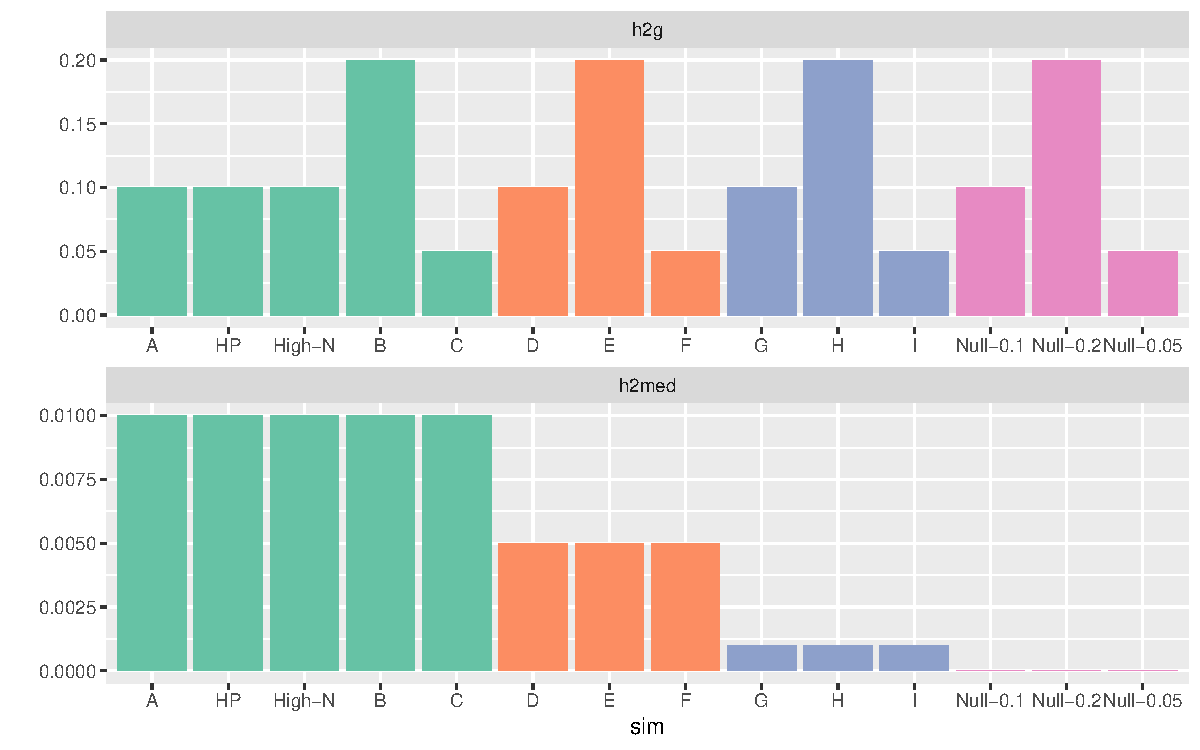
\includegraphics[width=.7\textwidth]{figs/sim_types}
  \caption{Diagram of the 12 types of \texttt{twas\_sim} simulations
    performed, varying eQTL $h^2$ (top row) and trait variance explained
    through gene expression (bottom row), with 20 replicates of each
    setting resulting in 240 simulations total. Results for simulation
    A are presented in Figure 2 in the main text, while results for
    the remaining 11 simulation settings follow in Supplementary
    Figures.}
\end{figure}

\begin{figure}[!ht]
  \centering
  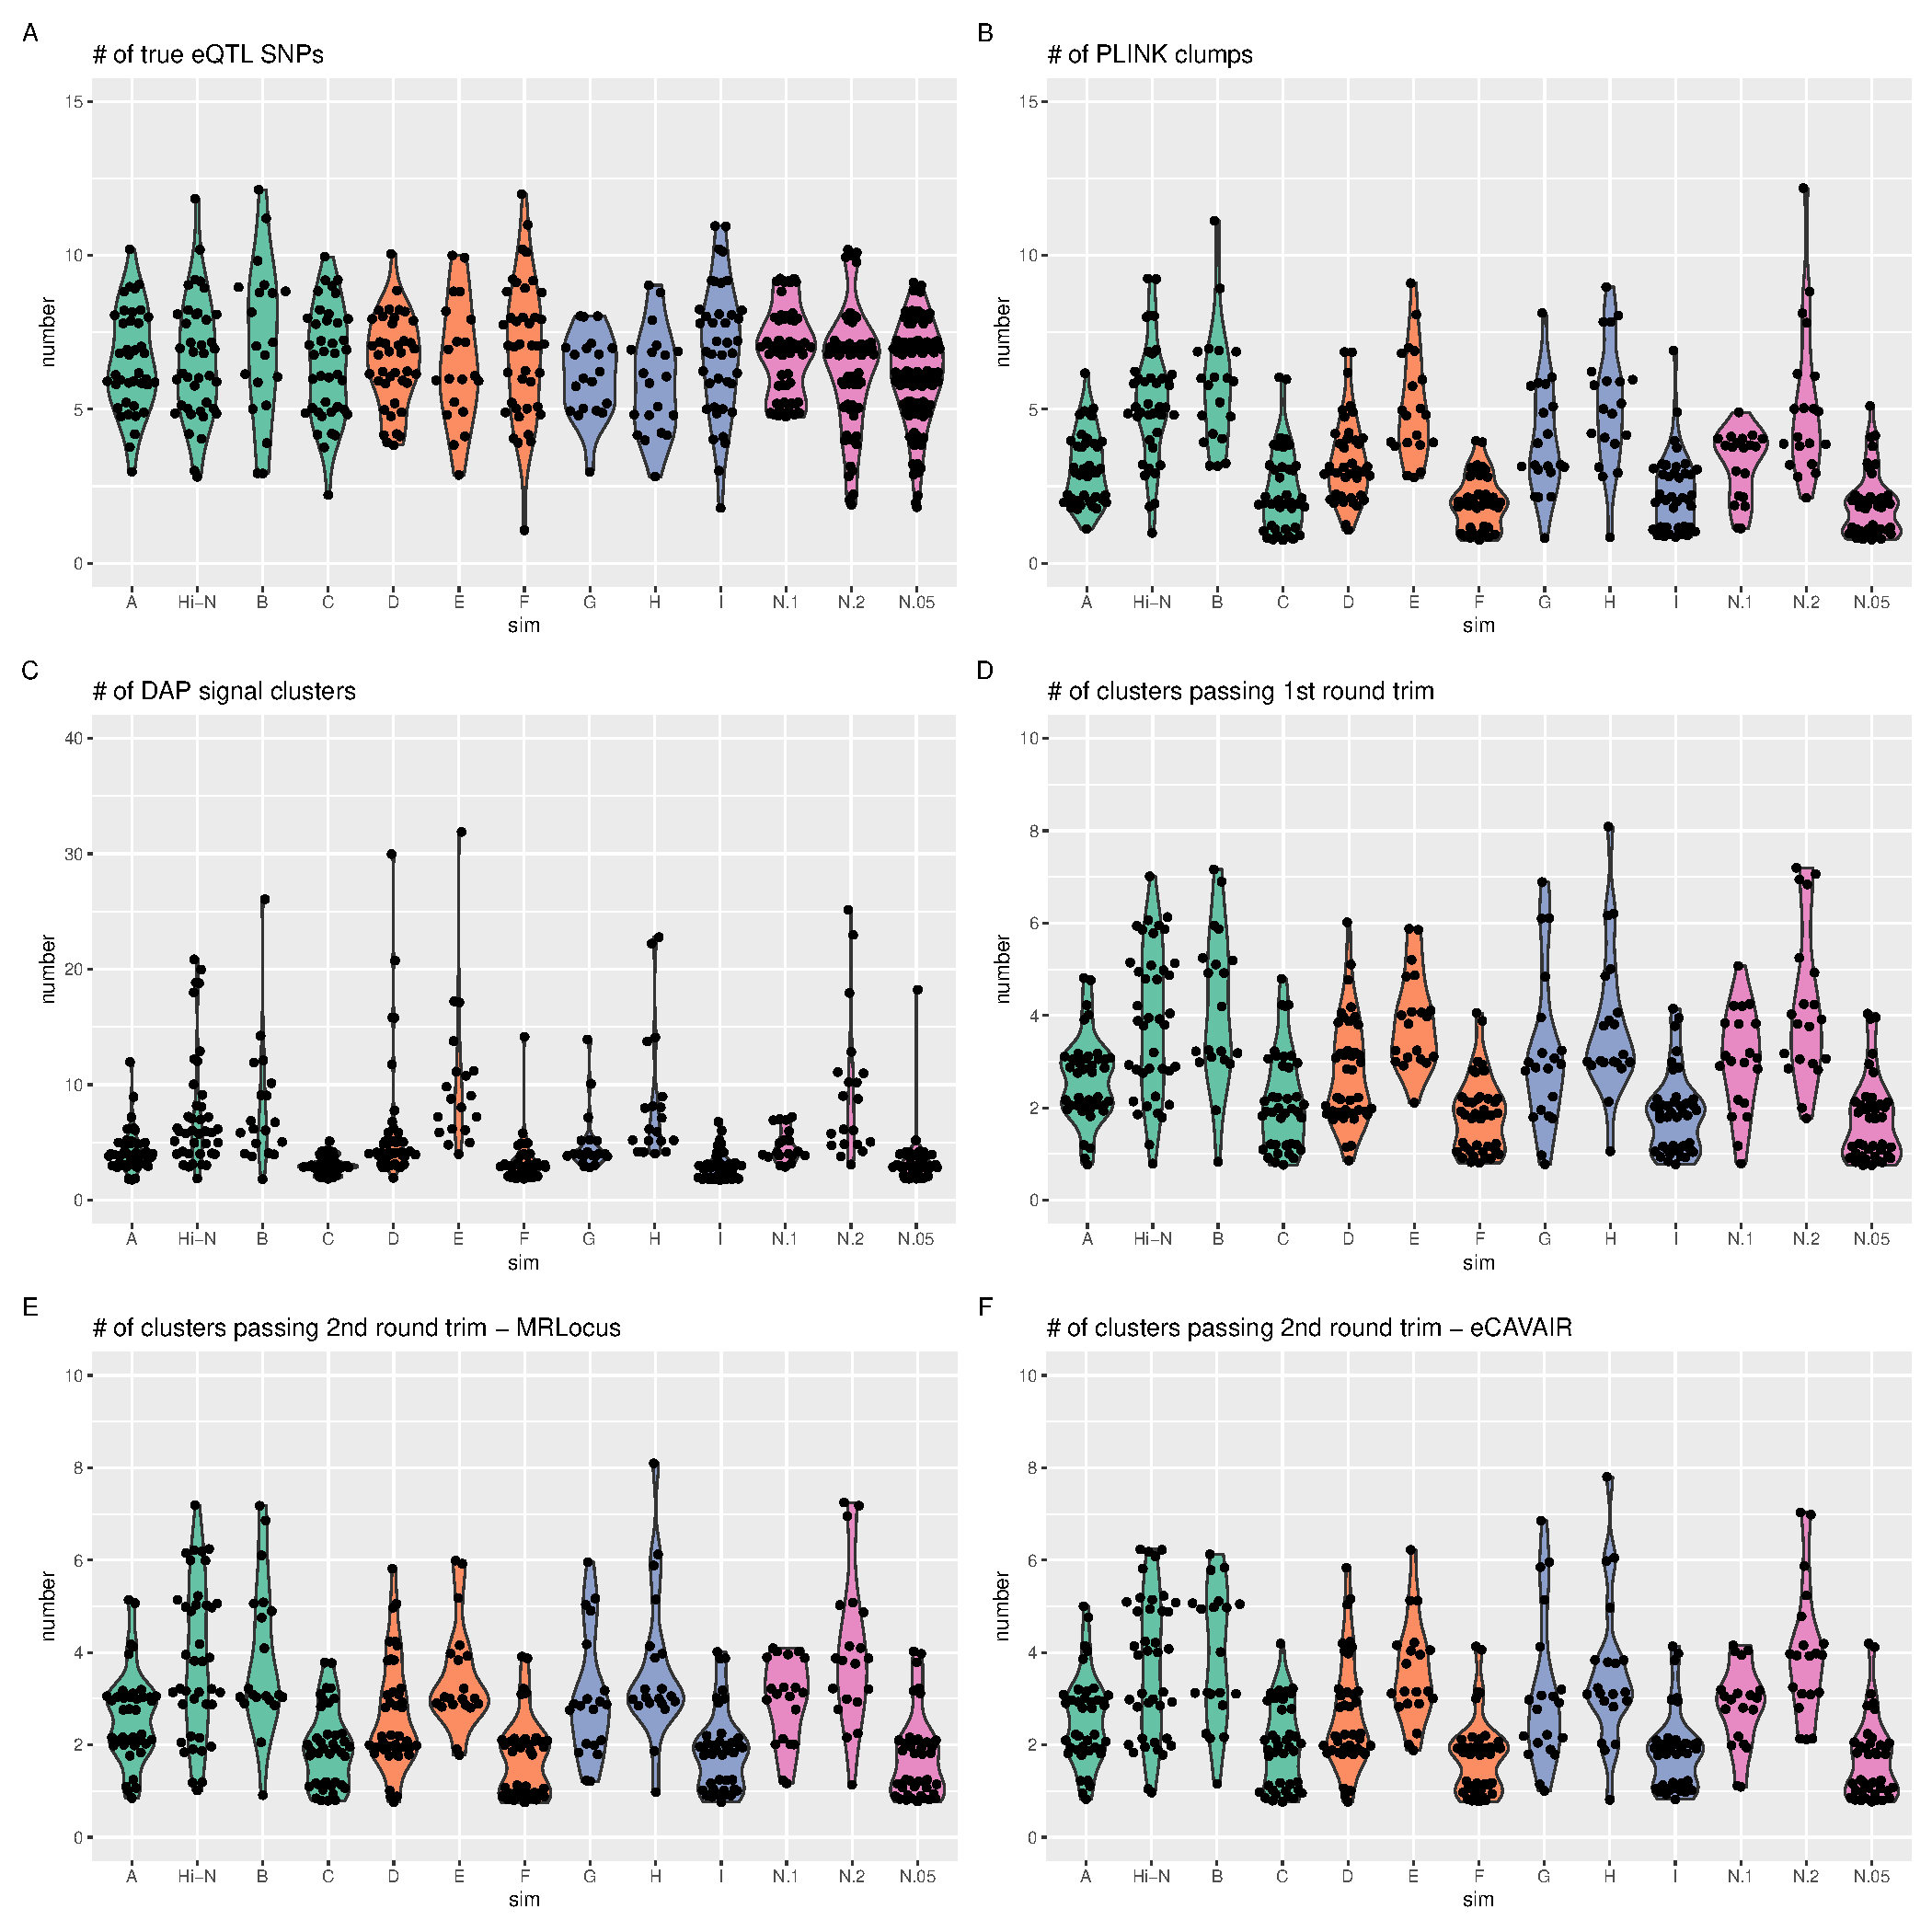
\includegraphics[width=\textwidth]{figs/sim_details}
  \caption{Number of (A) true causal eQTL SNPs, (B) PLINK clumps, and
    (C) DAP signal clusters per simulation.}
\end{figure}

\begin{figure}[!ht]
  \centering
  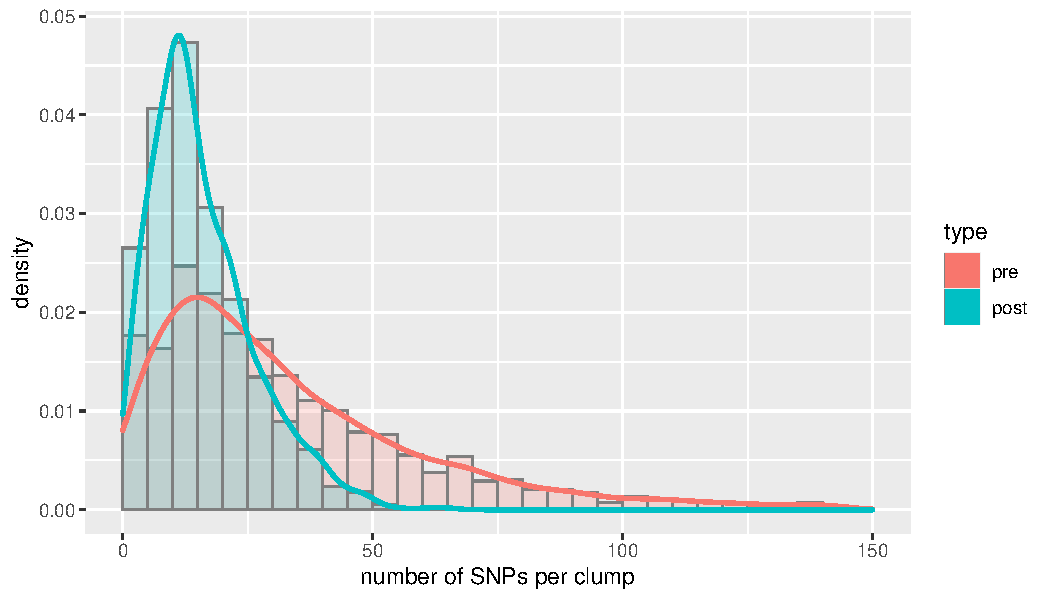
\includegraphics[width=.7\textwidth]{figs/snps-per-clump}
  \caption{SNPs per clump in the 240 simulations, before and after
    collapsing with MRLocus’ \texttt{collapseHighCorSNPs}
    function. The mean number of SNPs per clump was 19.9 and 8.8, and
    the median number of SNPs per clump was 15 and 8 (before and
    after, respectively).}
\end{figure}

\begin{figure}[!ht]
  \centering
  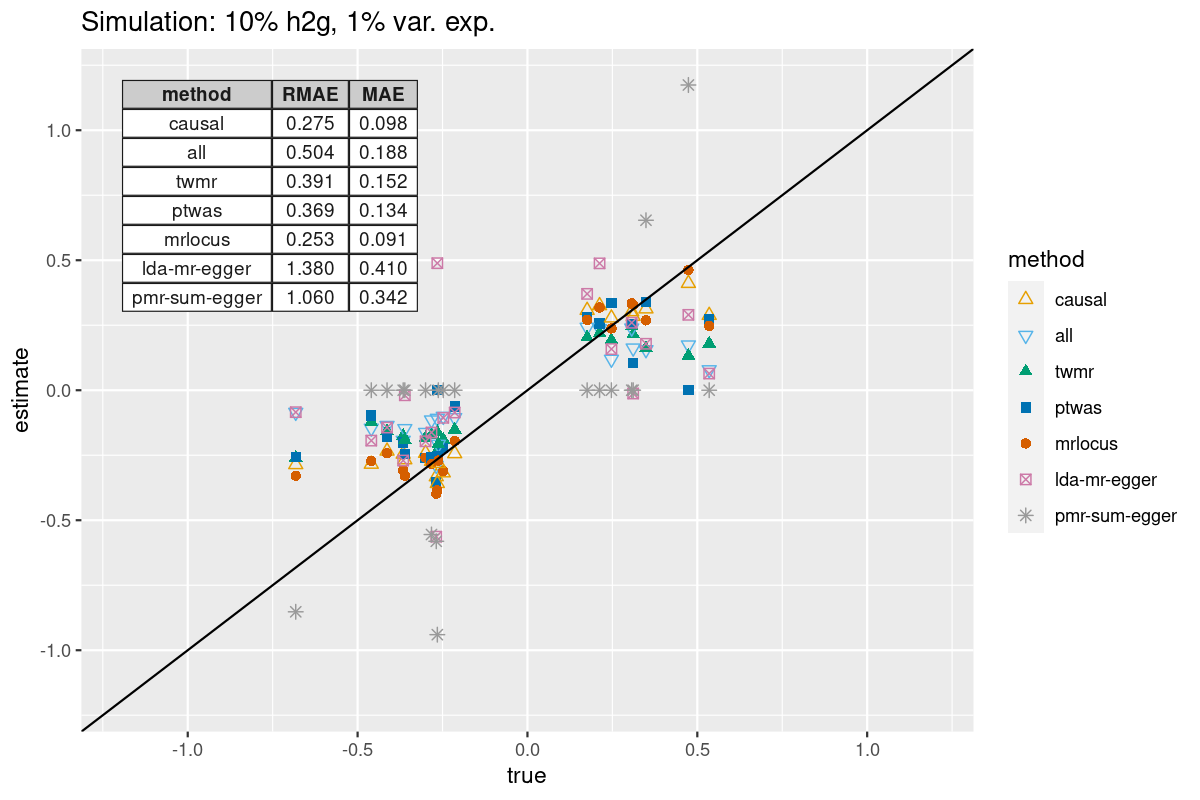
\includegraphics[width=.7\textwidth]{figs/sim1extra.png}
  \caption{Accuracy of gene-to-trait effect estimation in simulation
    A, including LDA-MR-Egger and PMR-Summary-Egger in
    comparisons. LDA-MR-Egger did not estimate SE for 6 of the 20
    simulations, and PMR-Summary-Egger did not provide an effect
    estimate for 14 of the 20 simulations.}
\end{figure}

\begin{figure}[!ht]
  \centering
  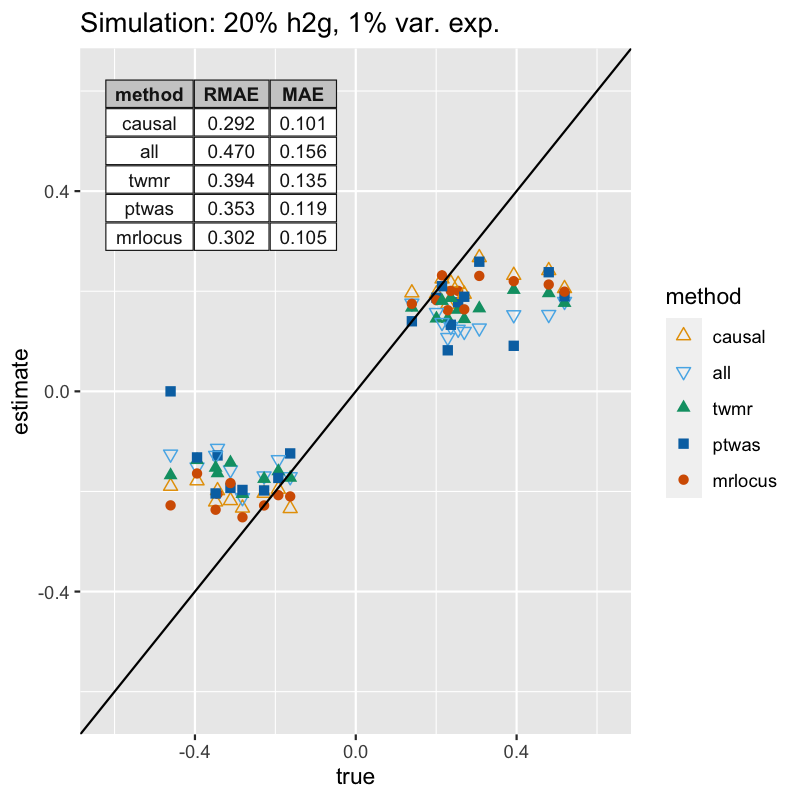
\includegraphics[width=.6\textwidth]{figs/sim3.png}
  \caption{Accuracy of gene-to-trait effect estimation in simulation B.}
\end{figure}

\begin{figure}[!ht]
  \centering
  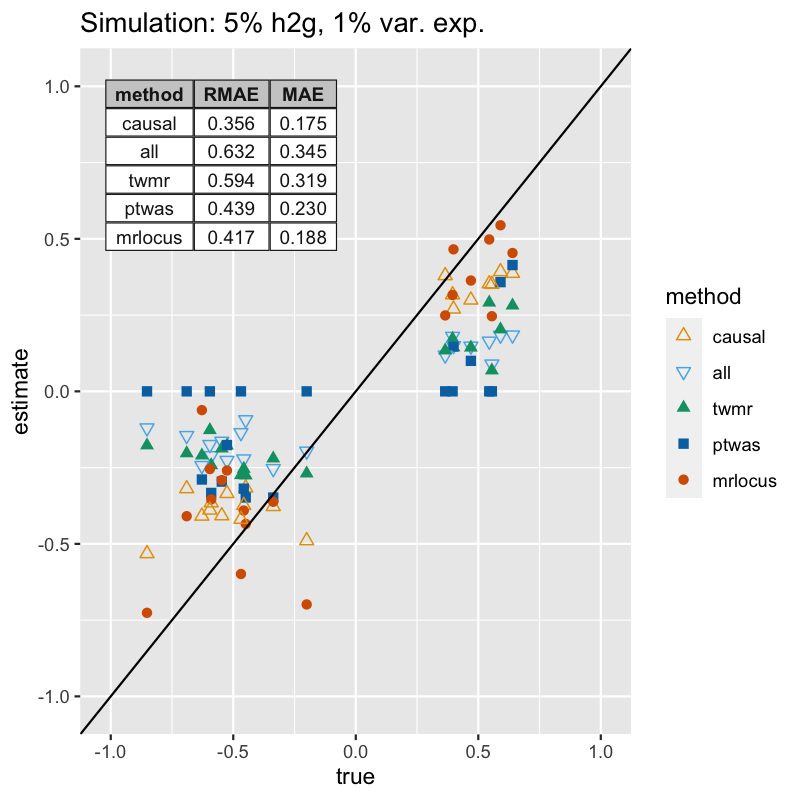
\includegraphics[width=.6\textwidth]{figs/sim2.png}
  \caption{Accuracy of gene-to-trait effect estimation in simulation C.}
\end{figure}

\begin{figure}[!ht]
  \centering
  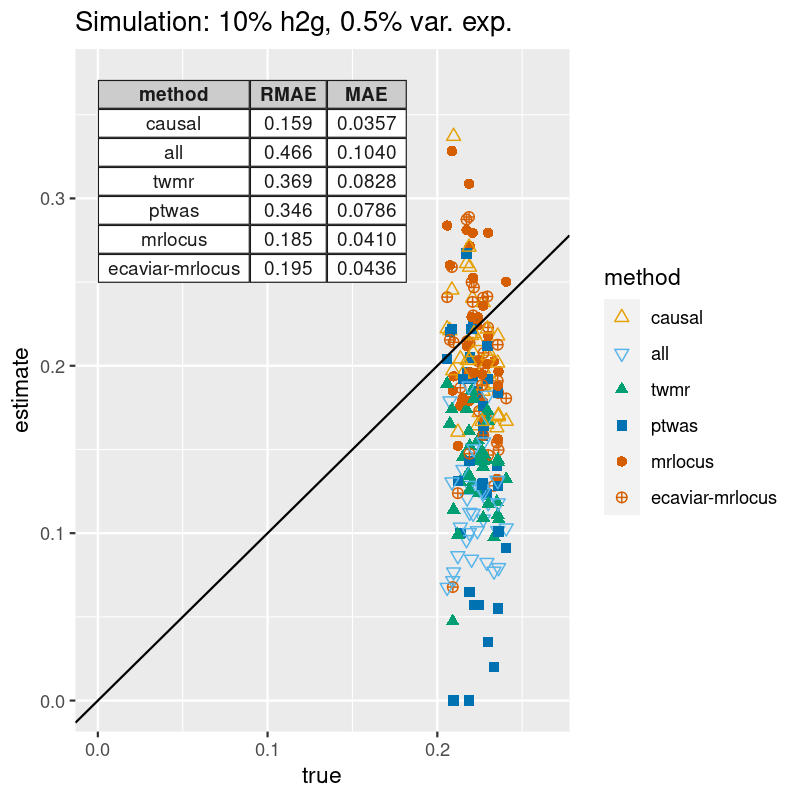
\includegraphics[width=.6\textwidth]{figs/sim4.png}
  \caption{Accuracy of gene-to-trait effect estimation in simulation D.}
\end{figure}

\begin{figure}[!ht]
  \centering
  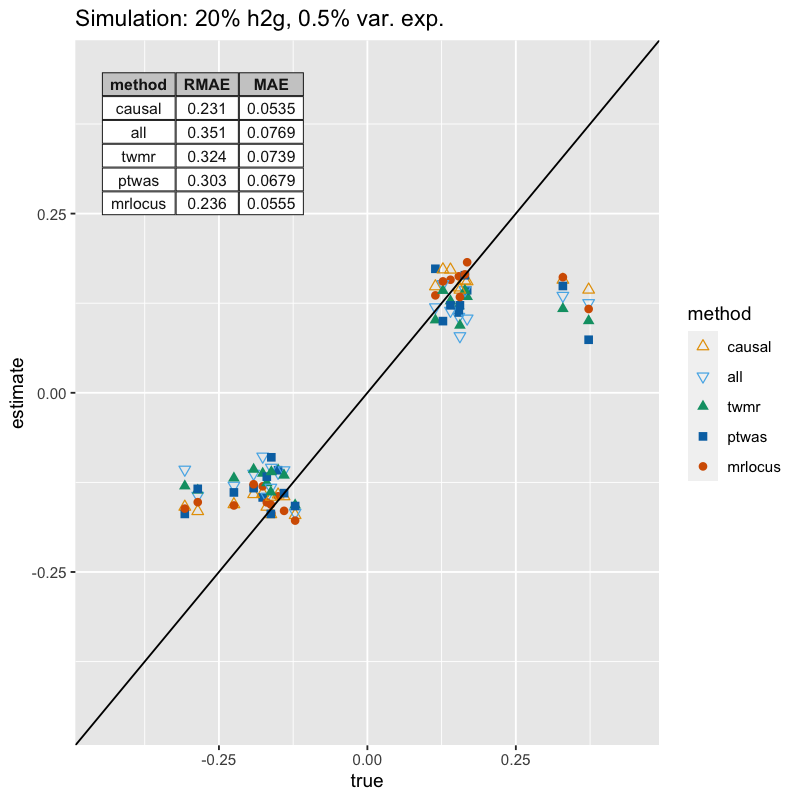
\includegraphics[width=.6\textwidth]{figs/sim6.png}
  \caption{Accuracy of gene-to-trait effect estimation in simulation E.}
\end{figure}

\begin{figure}[!ht]
  \centering
  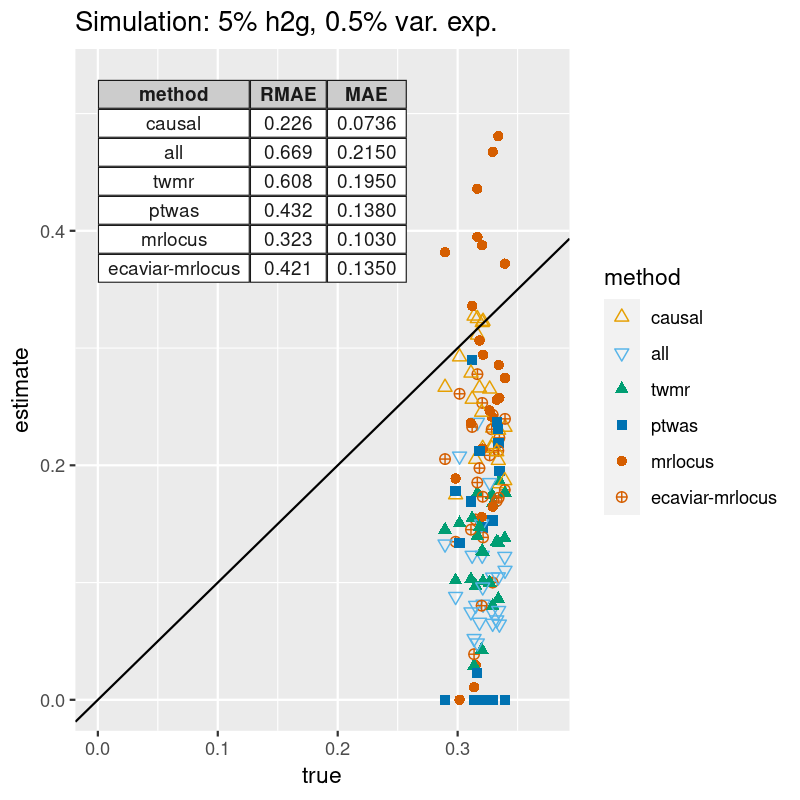
\includegraphics[width=.6\textwidth]{figs/sim8.png}
  \caption{Accuracy of gene-to-trait effect estimation in simulation F.}
\end{figure}

\begin{figure}[!ht]
  \centering
  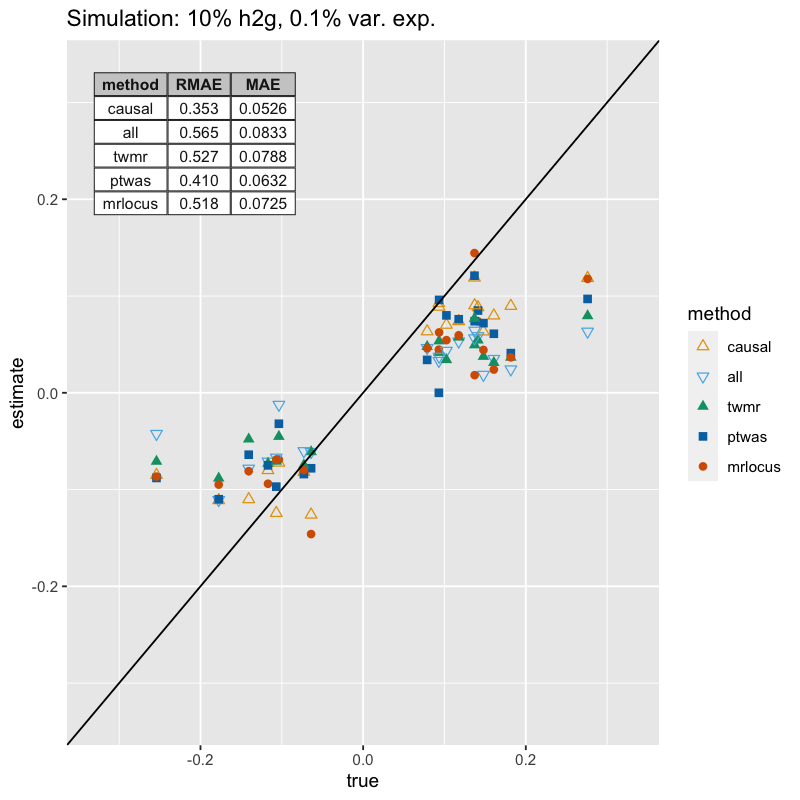
\includegraphics[width=.6\textwidth]{figs/sim5.png}
  \caption{Accuracy of gene-to-trait effect estimation in simulation G.}
\end{figure}

\begin{figure}[!ht]
  \centering
  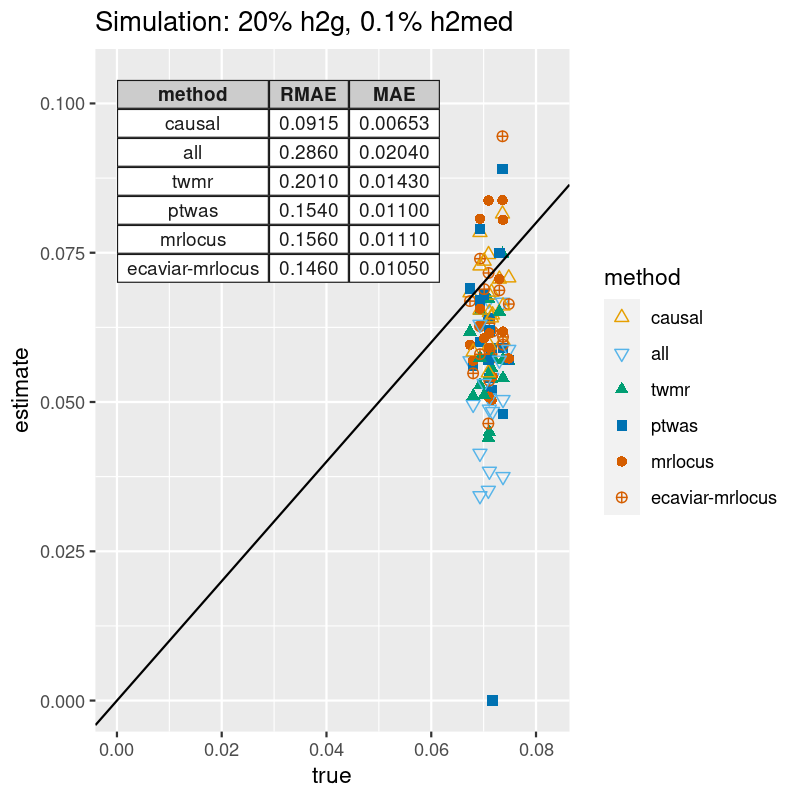
\includegraphics[width=.6\textwidth]{figs/sim7.png}
  \caption{Accuracy of gene-to-trait effect estimation in simulation H.}
\end{figure}

\begin{figure}[!ht]
  \centering
  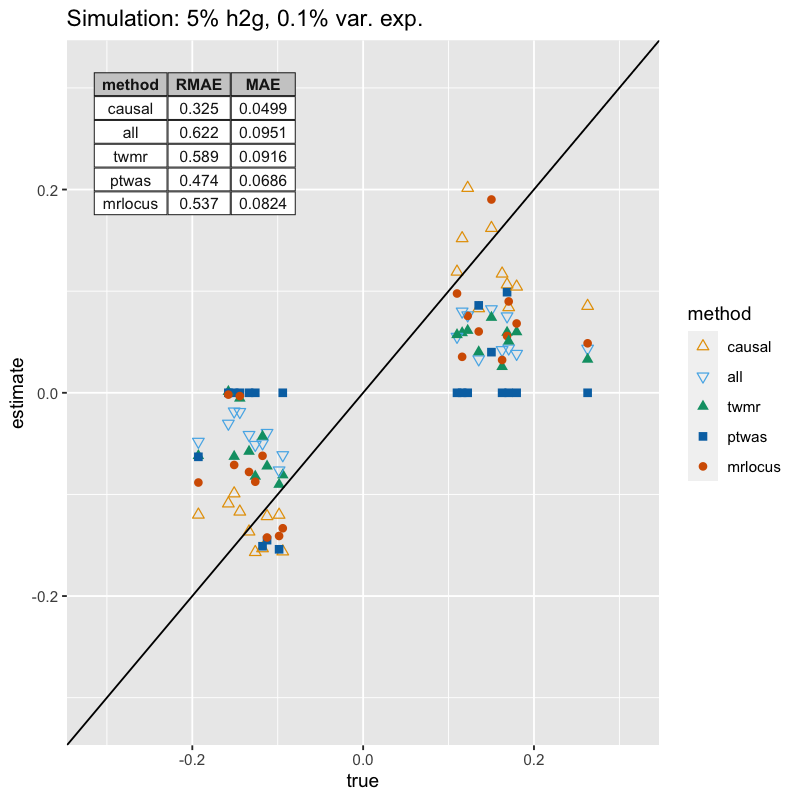
\includegraphics[width=.6\textwidth]{figs/sim9.png}
  \caption{Accuracy of gene-to-trait effect estimation in simulation I.}
\end{figure}

\begin{figure}[!ht]
  \centering
  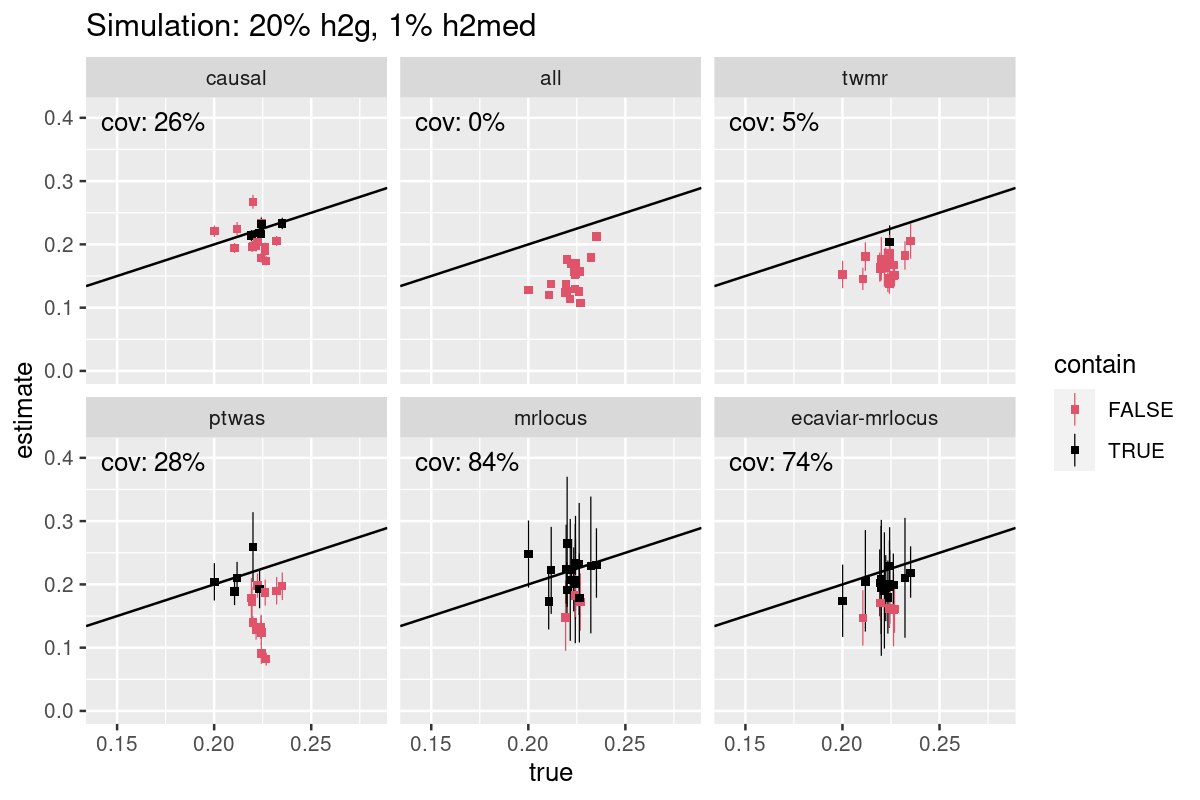
\includegraphics[width=.8\textwidth]{figs/cover3.png}
  \caption{Coverage of confidence or credible intervals for the
    gene-to-trait effect in simulation B.}
\end{figure}

\begin{figure}[!ht]
  \centering
  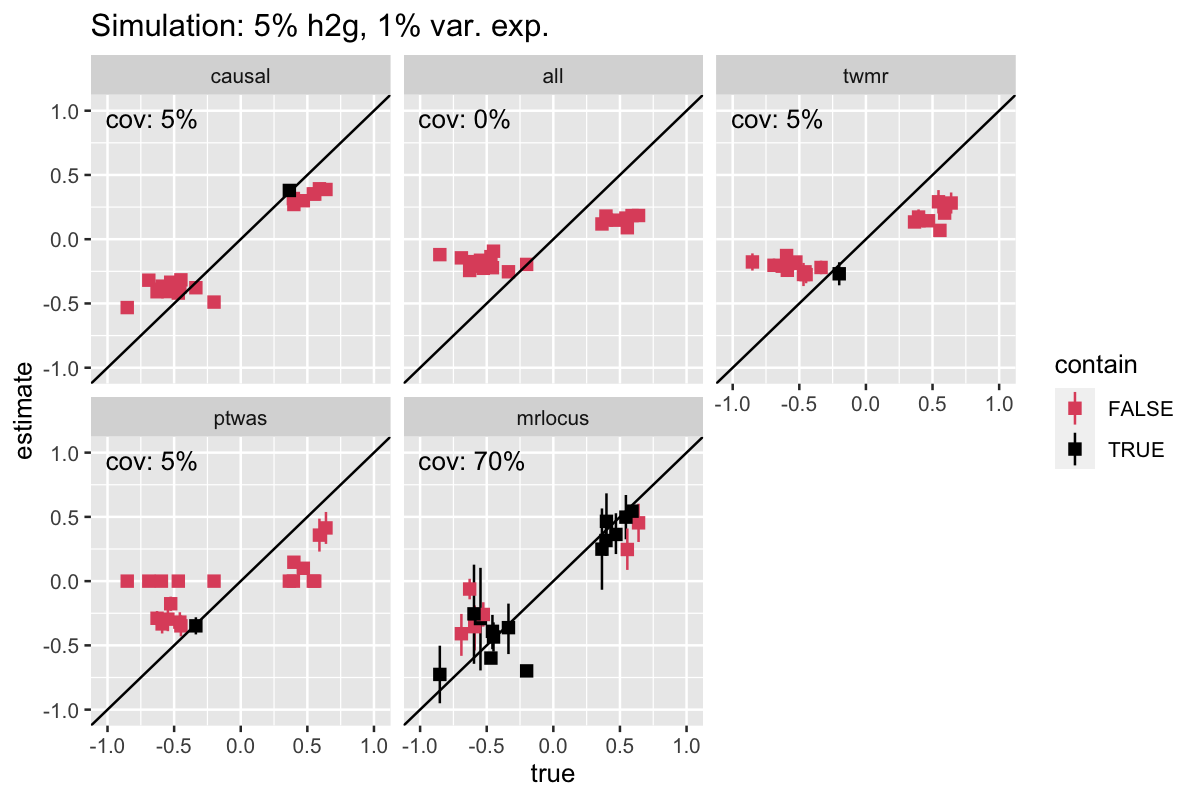
\includegraphics[width=.8\textwidth]{figs/cover2.png}
  \caption{Coverage of confidence or credible intervals for the
    gene-to-trait effect in simulation C.}
\end{figure}

\begin{figure}[!ht]
  \centering
  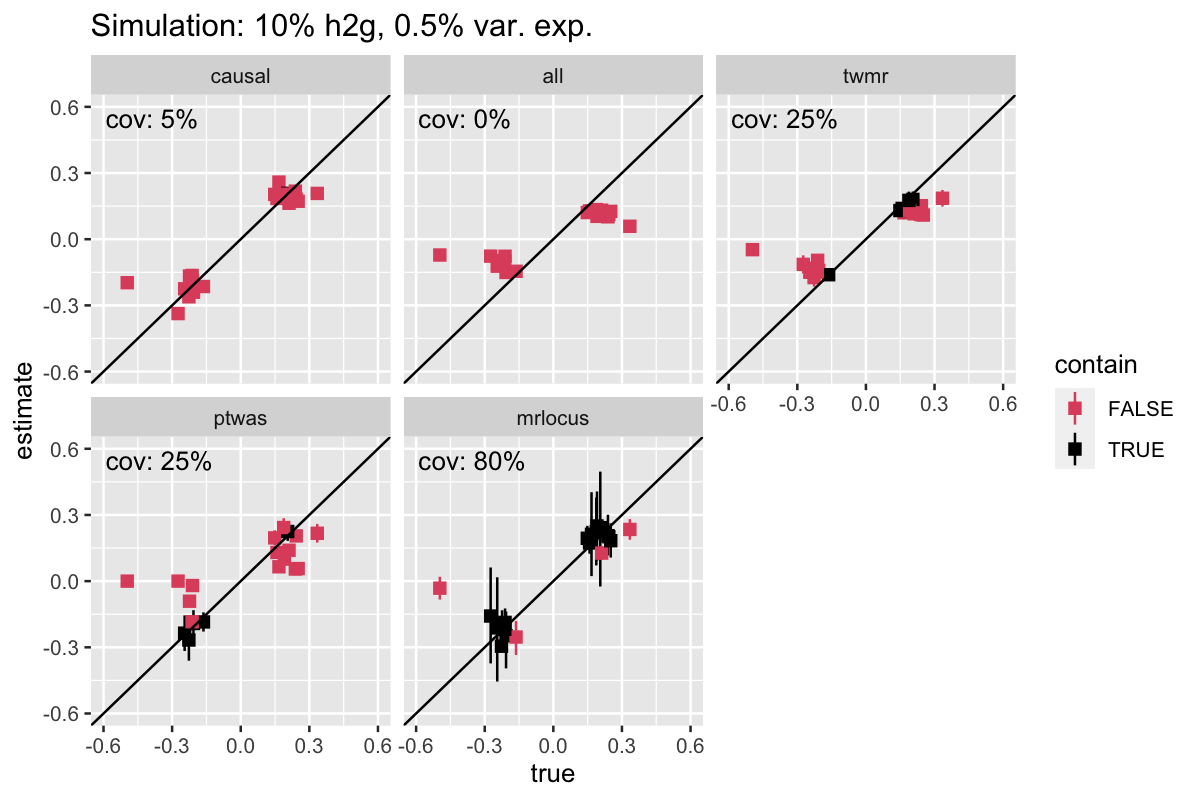
\includegraphics[width=.8\textwidth]{figs/cover4.png}
  \caption{Coverage of confidence or credible intervals for the
    gene-to-trait effect in simulation D.}
\end{figure}

\begin{figure}[!ht]
  \centering
  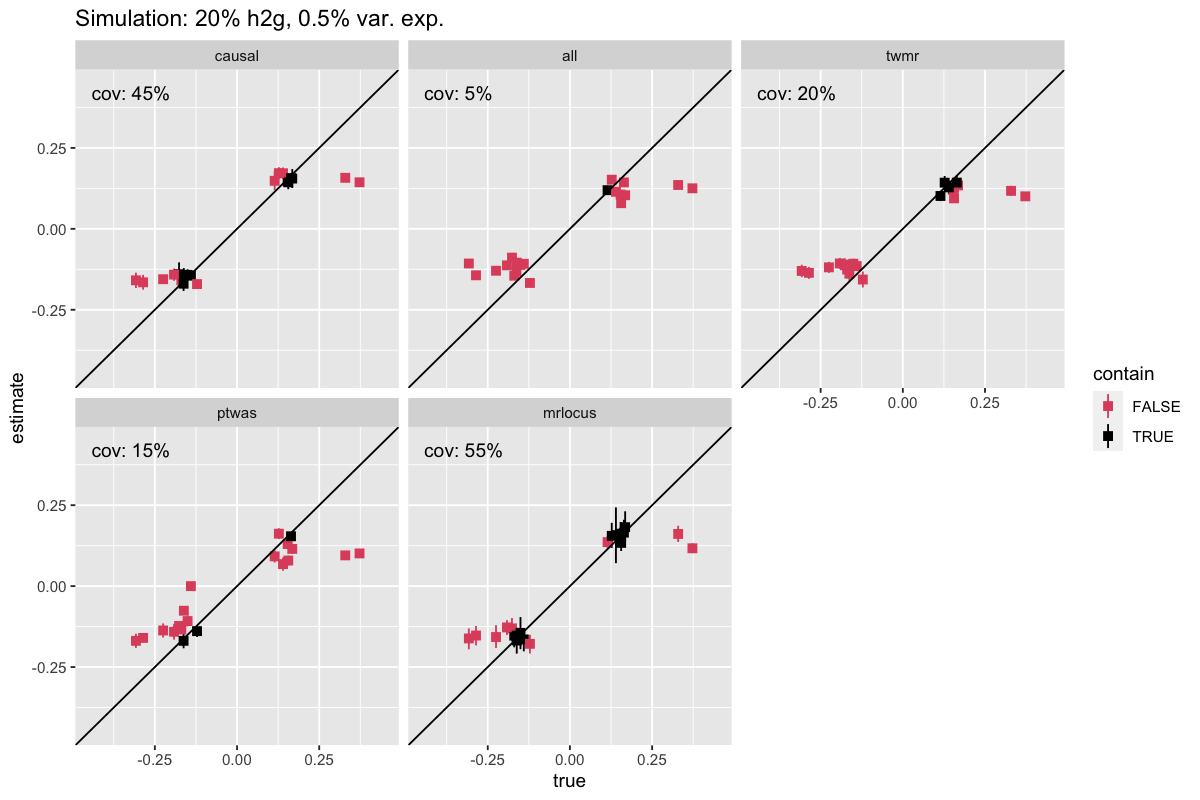
\includegraphics[width=.8\textwidth]{figs/cover6.png}
  \caption{Coverage of confidence or credible intervals for the
    gene-to-trait effect in simulation E.}
\end{figure}

\begin{figure}[!ht]
  \centering
  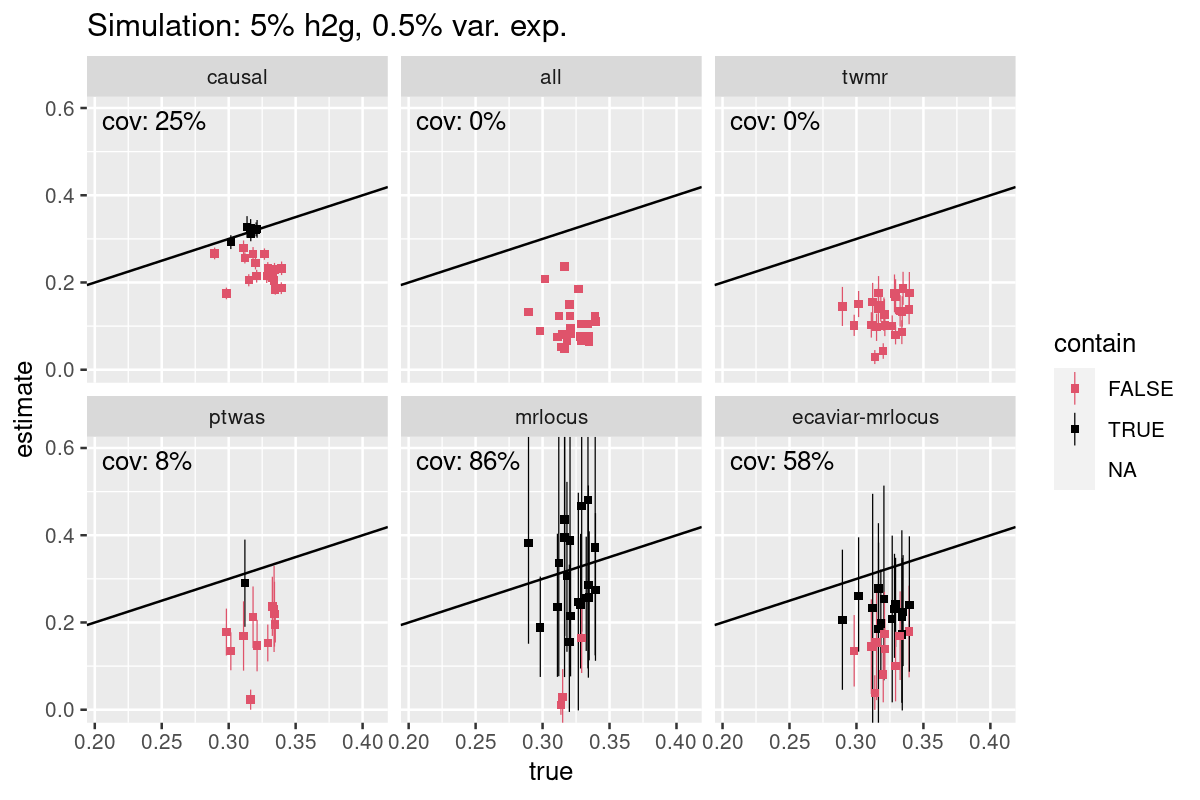
\includegraphics[width=.8\textwidth]{figs/cover8.png}
  \caption{Coverage of confidence or credible intervals for the
    gene-to-trait effect in simulation F.}
\end{figure}

\begin{figure}[!ht]
  \centering
  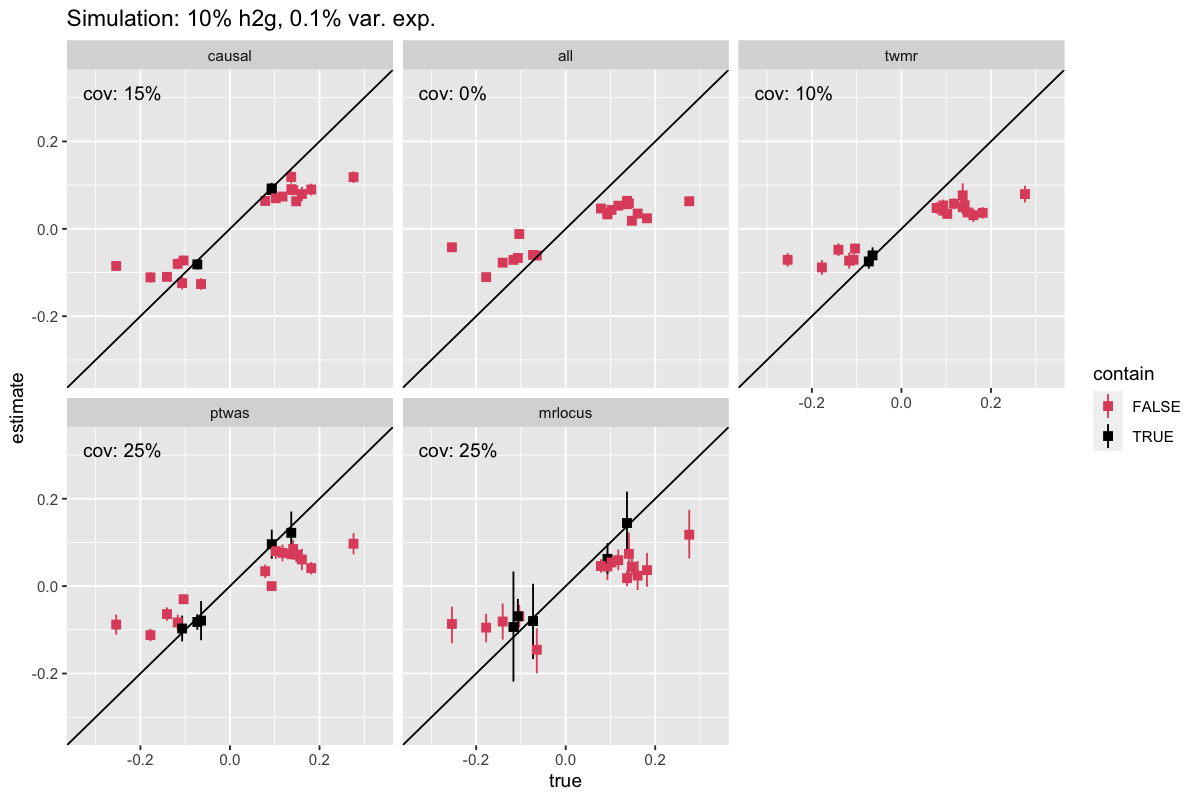
\includegraphics[width=.8\textwidth]{figs/cover5.png}
  \caption{Coverage of confidence or credible intervals for the
    gene-to-trait effect in simulation G.}
\end{figure}

\begin{figure}[!ht]
  \centering
  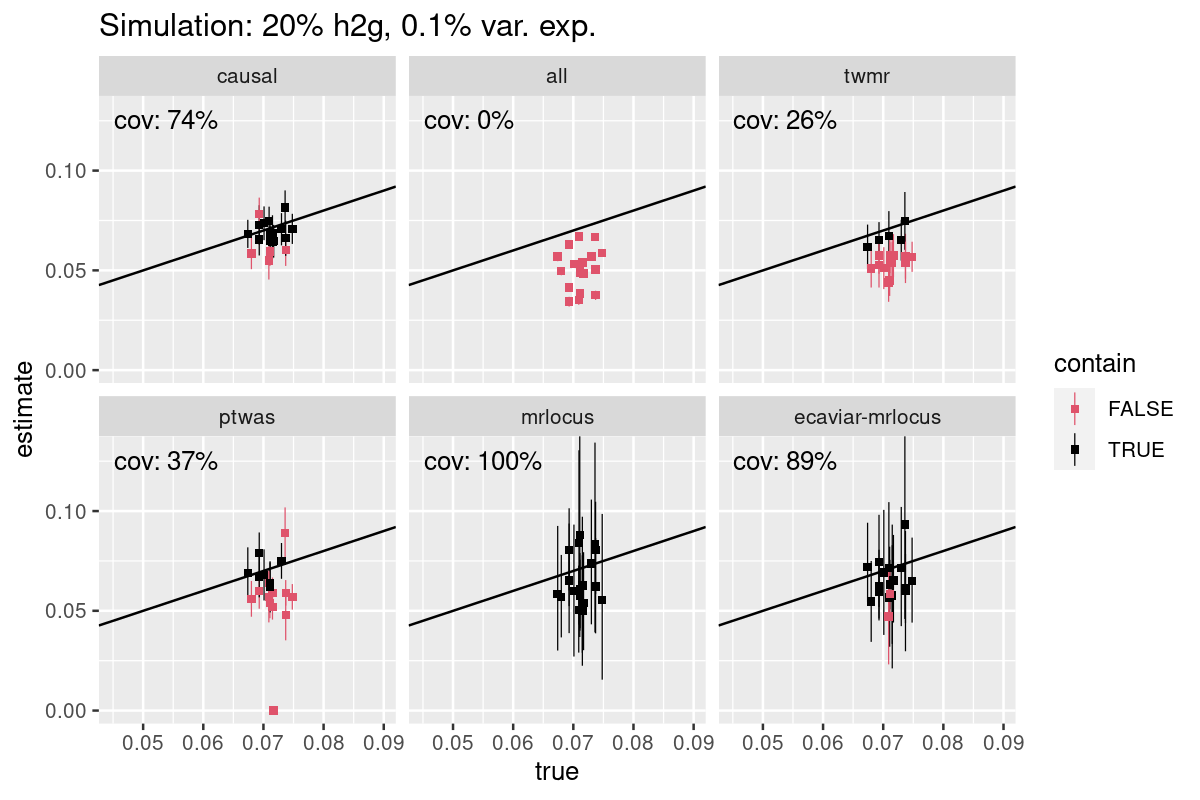
\includegraphics[width=.8\textwidth]{figs/cover7.png}
  \caption{Coverage of confidence or credible intervals for the
    gene-to-trait effect in simulation H.}
\end{figure}

\begin{figure}[!ht]
  \centering
  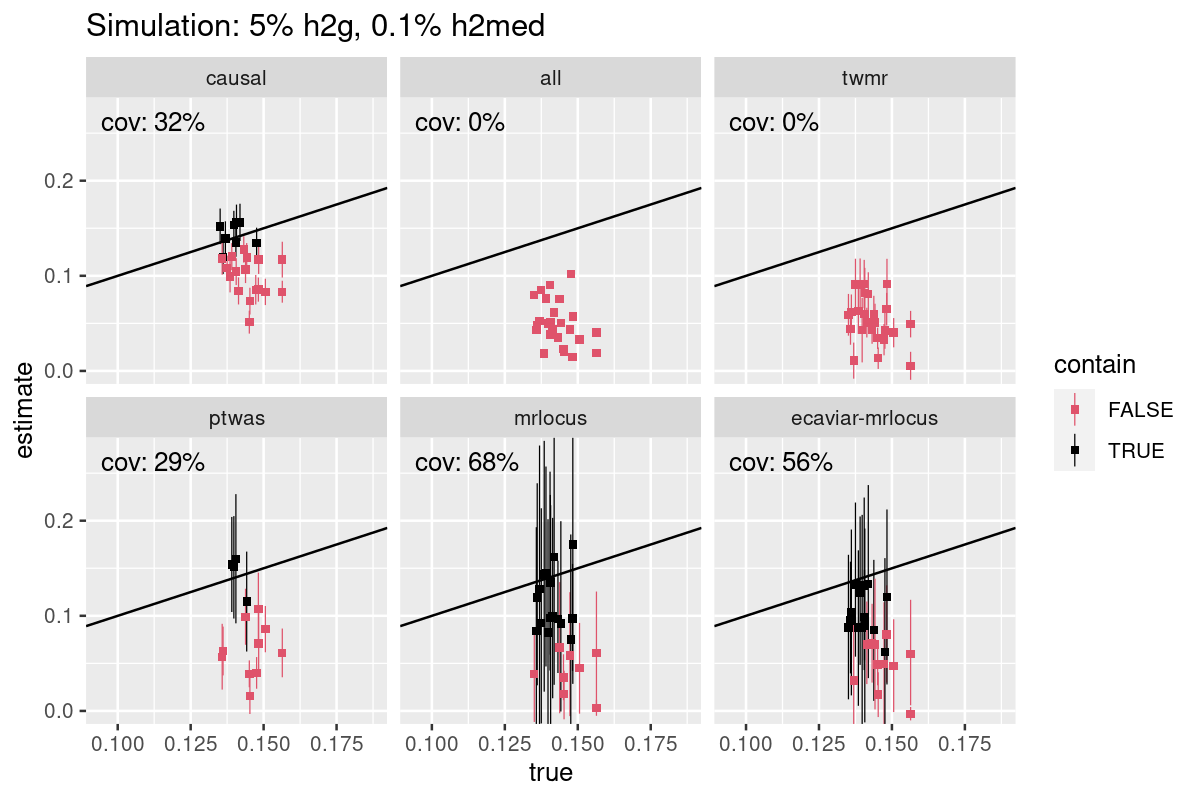
\includegraphics[width=.8\textwidth]{figs/cover9.png}
  \caption{Coverage of confidence or credible intervals for the
    gene-to-trait effect in simulation I.}
\end{figure}

\begin{figure}[!ht]
  \centering
  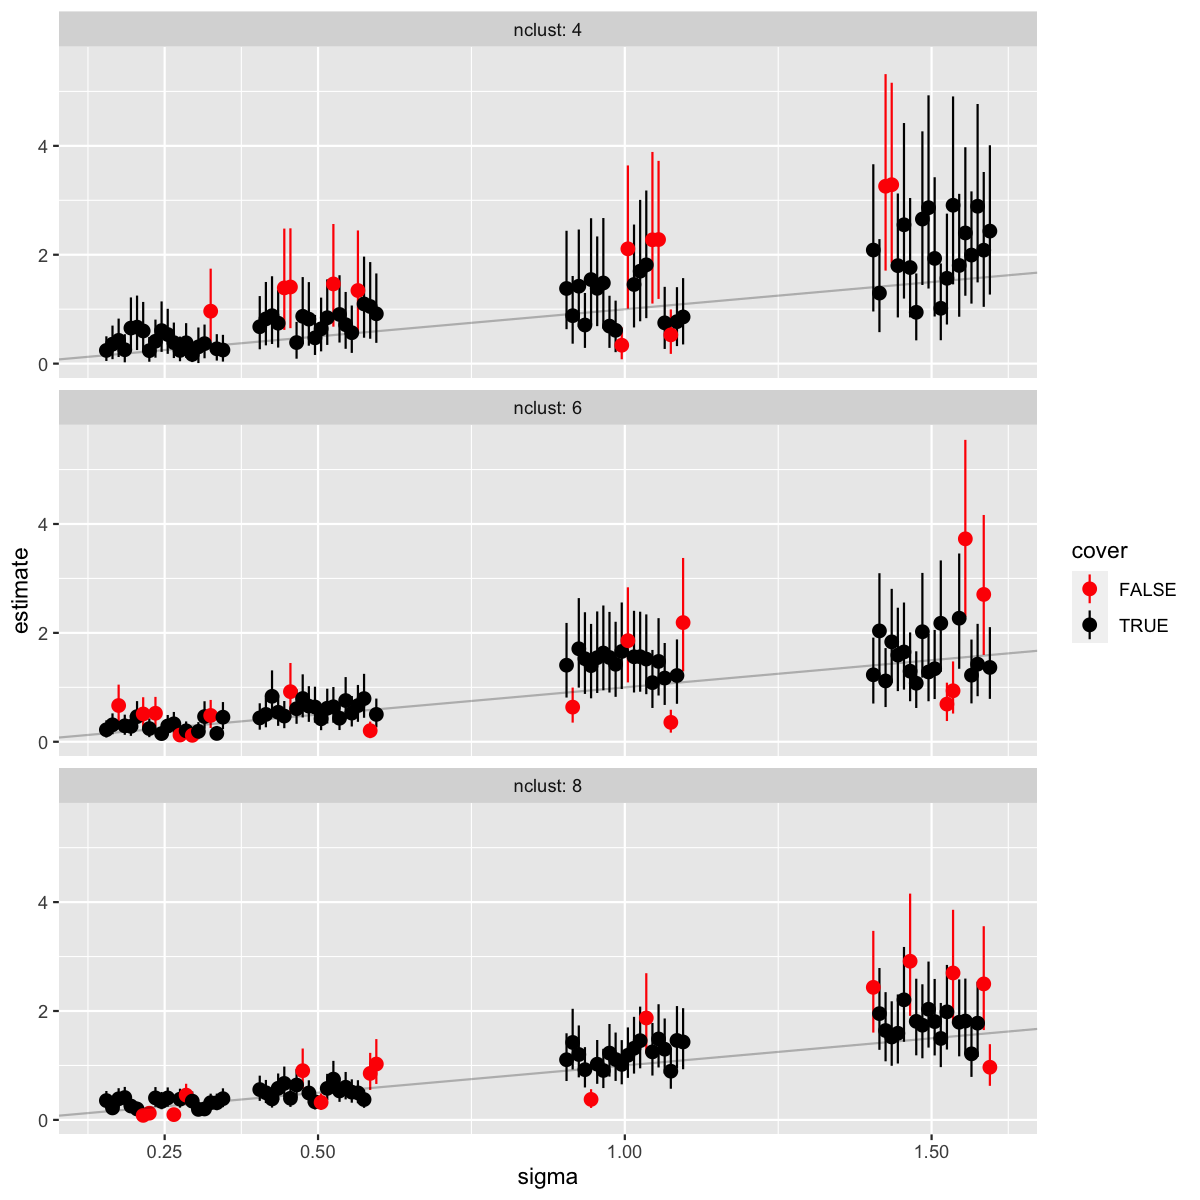
\includegraphics[width=\textwidth]{figs/sigma_est.png}
  \caption{Simulation assessing MRLocus' estimation of the scale of
    dispersion ($\sigma$) across independent signal
    clusters. The summary statistics for eQTL and GWAS were generated from
    a multivariate normal distribution as in the eCAVIAR model, using
    a simulated LD matrix. The true slope ($\alpha$) was set to 1, the
    true $\sigma$ varied from 0.25 to 1 in increments of 0.25
    (x-axis), and the number of LD-independent clusters varied between
    4, 6, and 8 (left, middle, and right panels), with 10 iterations
    per setting (plotted with spacing to avoid overplotting). The
    posterior mean is indicated with a dot, while 80\% quantile-based
    credible intervals and their coverage of the true value are
    indicated with the line and its color. The simulation script is
    included within the MRLocus package test directory, as an R
    script \texttt{"test\_sigma.R"}.}
\end{figure}

\begin{figure}[!ht]
  \centering
  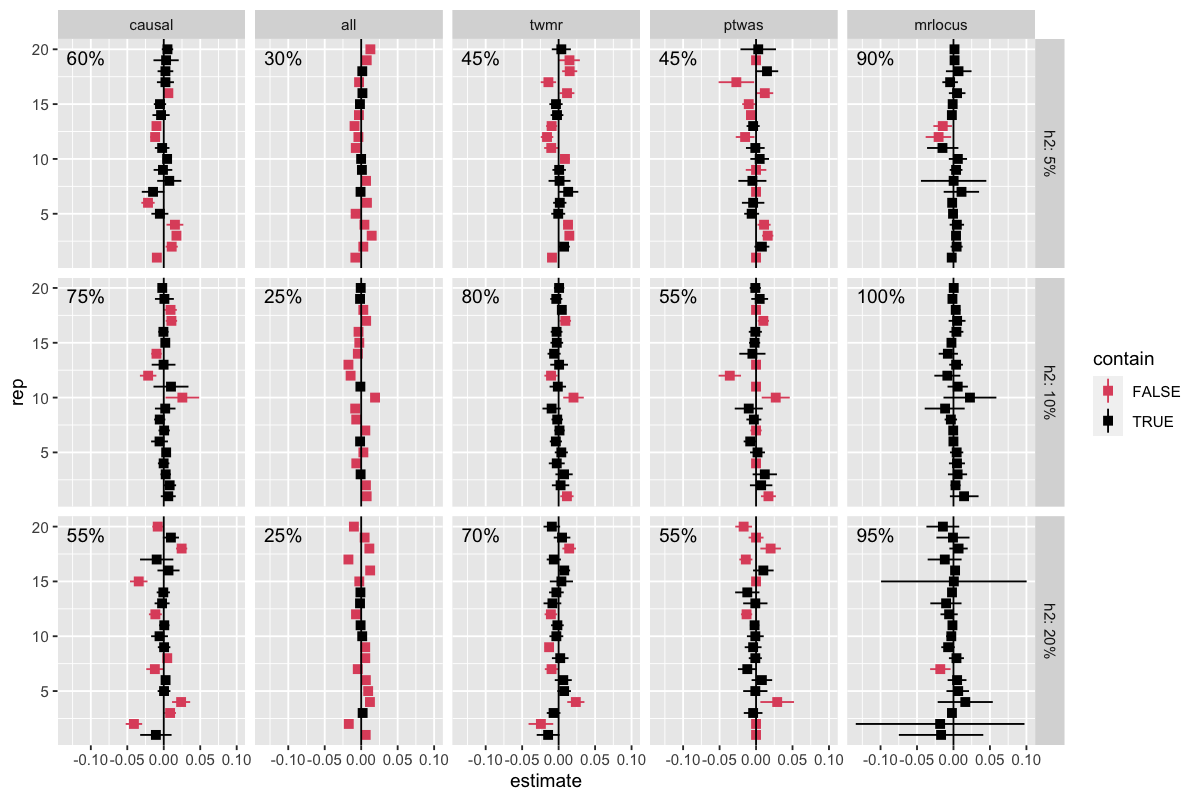
\includegraphics[width=\textwidth]{figs/nullplot.png}
  \caption{Coverage of confidence or credible intervals for the 3 null
    simulation settings.}
\end{figure}

\begin{figure}[!ht]
  \centering
  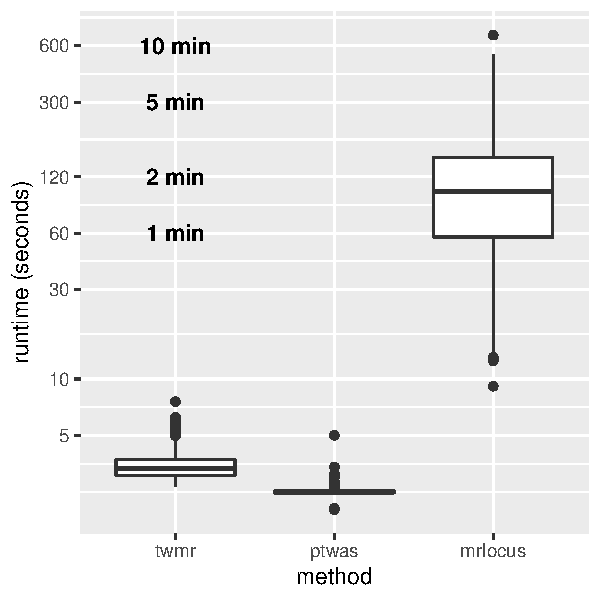
\includegraphics[width=.7\textwidth]{figs/runtime}
  \caption{Runtime for TWMR, PTWAS, and MRLocus on the 240
    simulations. The runtime for a single locus using a single core is
    shown on the y-axis (log scale).}
\end{figure}

\begin{figure}[!ht]
  \centering
  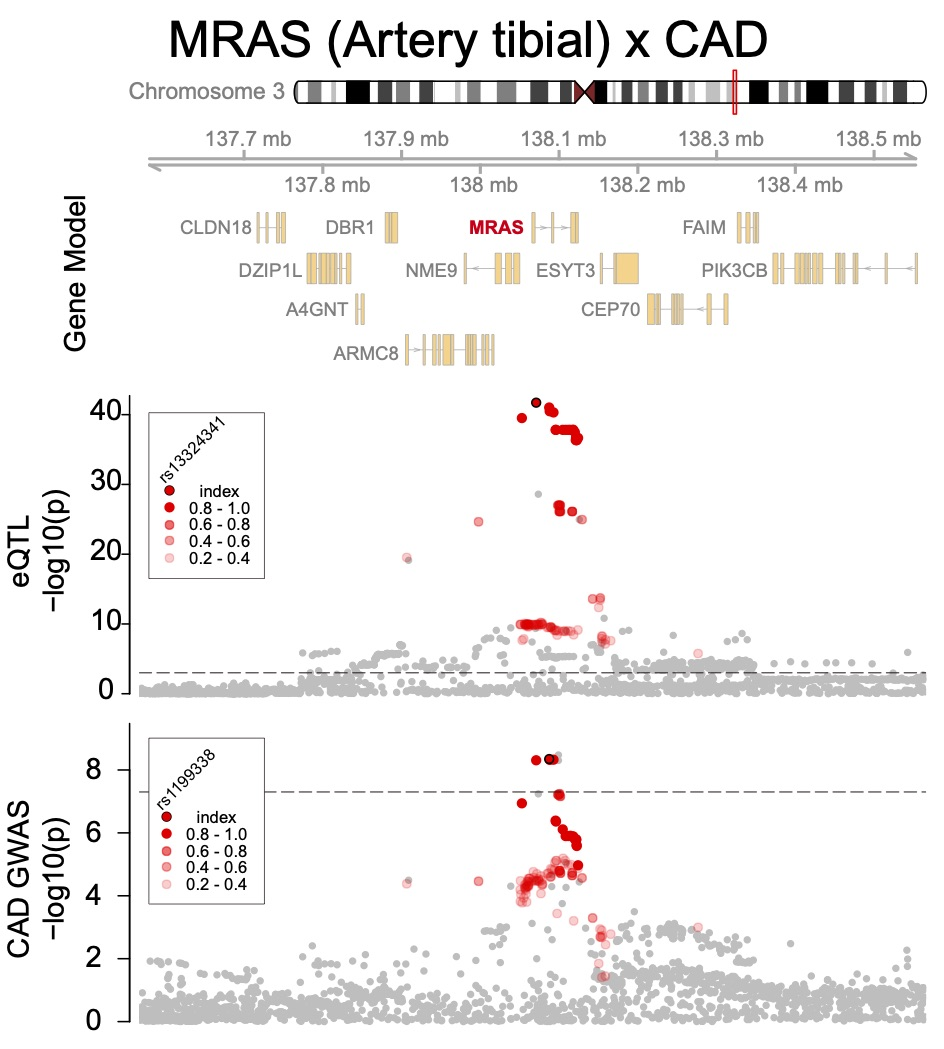
\includegraphics[width=.7\textwidth]{figs/region_mras.jpg}
  \caption{Colocalized signals in the \emph{MRAS} region. From top panel to
    bottom, gene model (NCBI Refseq), eQTL for MRAS in artery tibial
    (GTEx; N = 663) and CAD association within CARDIoGRAMplusC4D
    (\Ncase = 60,801 and \Ncontrol = 123,504) (M. Nikpay et al.,
    2015). LD was calculated to independent SNPs within 1KG EUR and
    colored accordingly. Symbols indicate independent co-localized
    ($r^2 > 0.4$) eQTL-GWAS pairs. Dashed line indicates a significance
    threshold at p = 0.001 or p = 5x$10^{-8}$ for eQTL and GWAS
    respectively.}
\end{figure}

\begin{figure}[!ht]
  \centering
  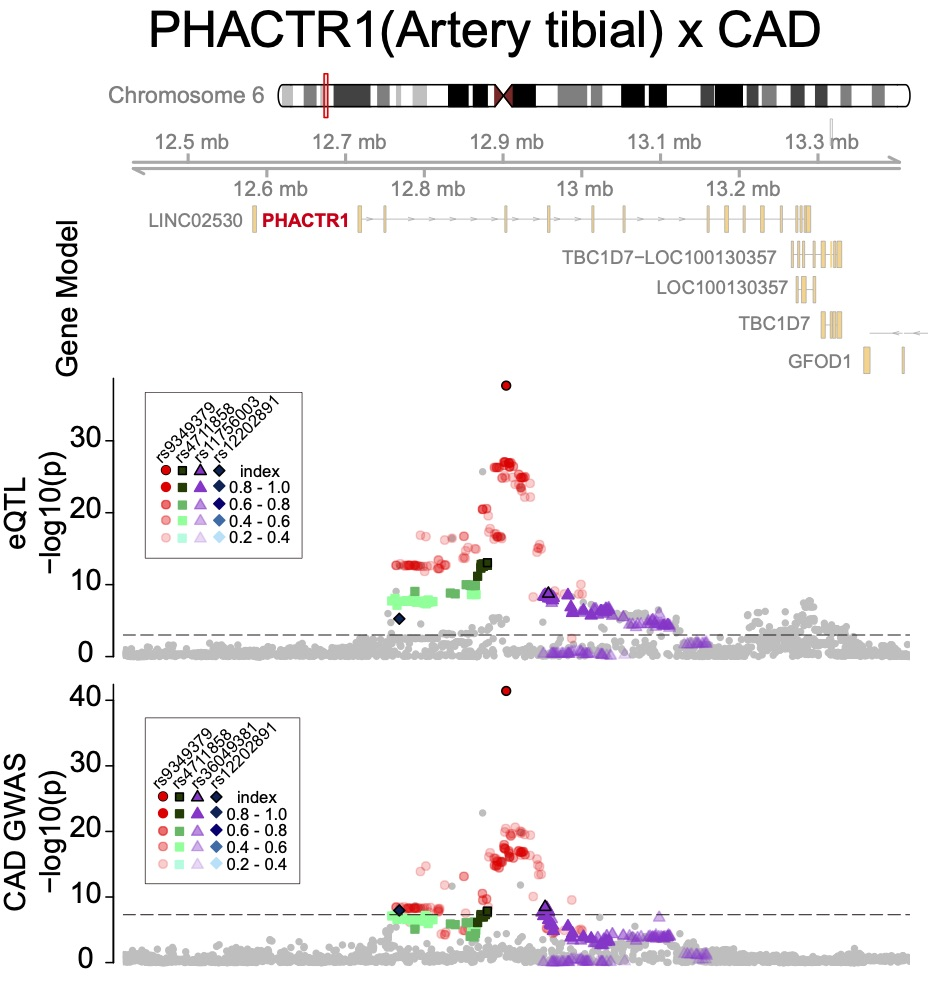
\includegraphics[width=.7\textwidth]{figs/region_phactr1.jpg}
  \caption{Colocalized signals in the \emph{PHACTR1} region. From top
    panel to bottom, gene model (NCBI Refseq), eQTL for PHACTR1 in
    artery tibial (GTEx; N = 663) and CAD association within
    CARDIoGRAMplusC4D (\Ncase = 60,801 and \Ncontrol = 123,504)
    (M. Nikpay et al., 2015). LD was calculated to independent SNPs
    within 1KG EUR and colored accordingly. Symbols indicate
    independent co-localized ($r^2 > 0.4$) eQTL-GWAS pairs. Dashed
    line indicates a significance threshold at p = 0.001 or p =
    5x$10^{-8}$ for eQTL and GWAS respectively.} 
\end{figure}

\begin{figure}[!ht]
  \centering
  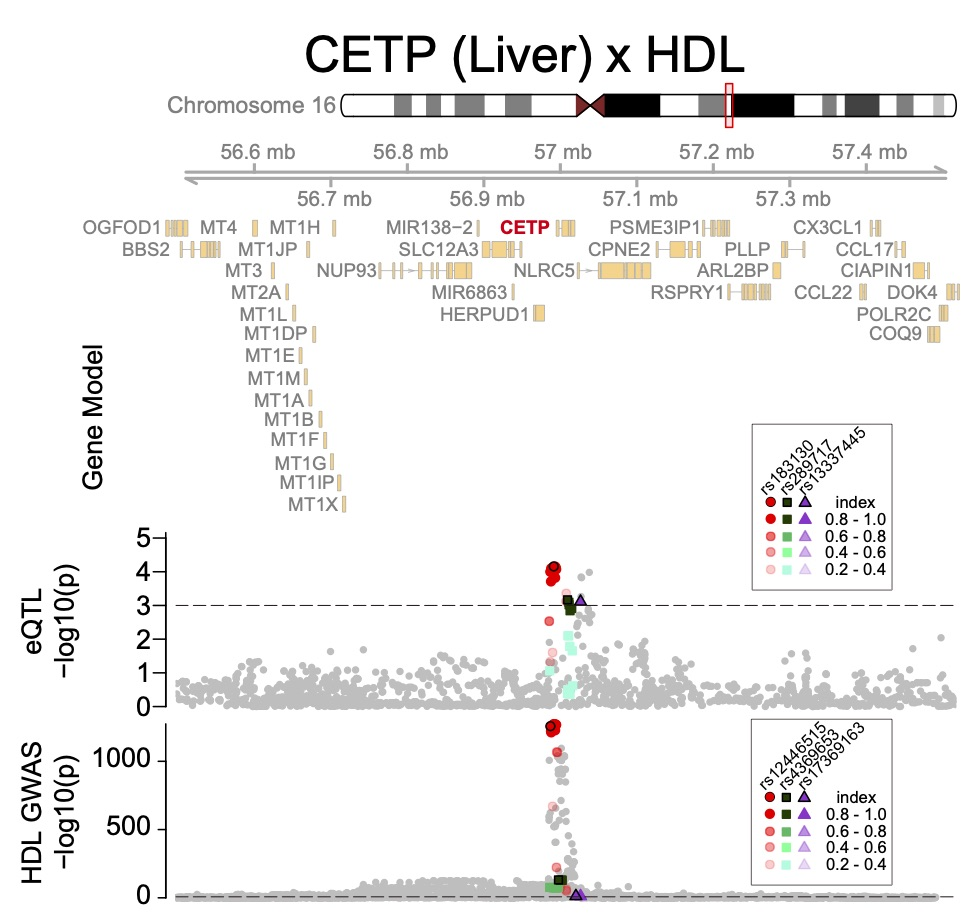
\includegraphics[width=.7\textwidth]{figs/region_cetp.jpg}
  \caption{Colocalized signals in the \emph{CETP} region. From top
    panel to bottom, gene model (NCBI Refseq), eQTL for CETP in liver
    (N = 588) (Strunz et al., 2018) and HDL association within UKBB (N
    = 315,133). LD was calculated to independent SNPs within 1KG EUR
    and colored accordingly. Symbols indicate independent co-localized
    ($r^2 > 0.4$) eQTL-GWAS pairs. Dashed line indicates a significance
    threshold at p = 0.001 or p = 5x$10^{-8}$ for eQTL and GWAS
    respectively.} 
\end{figure}

\begin{figure}[!ht]
  \centering
  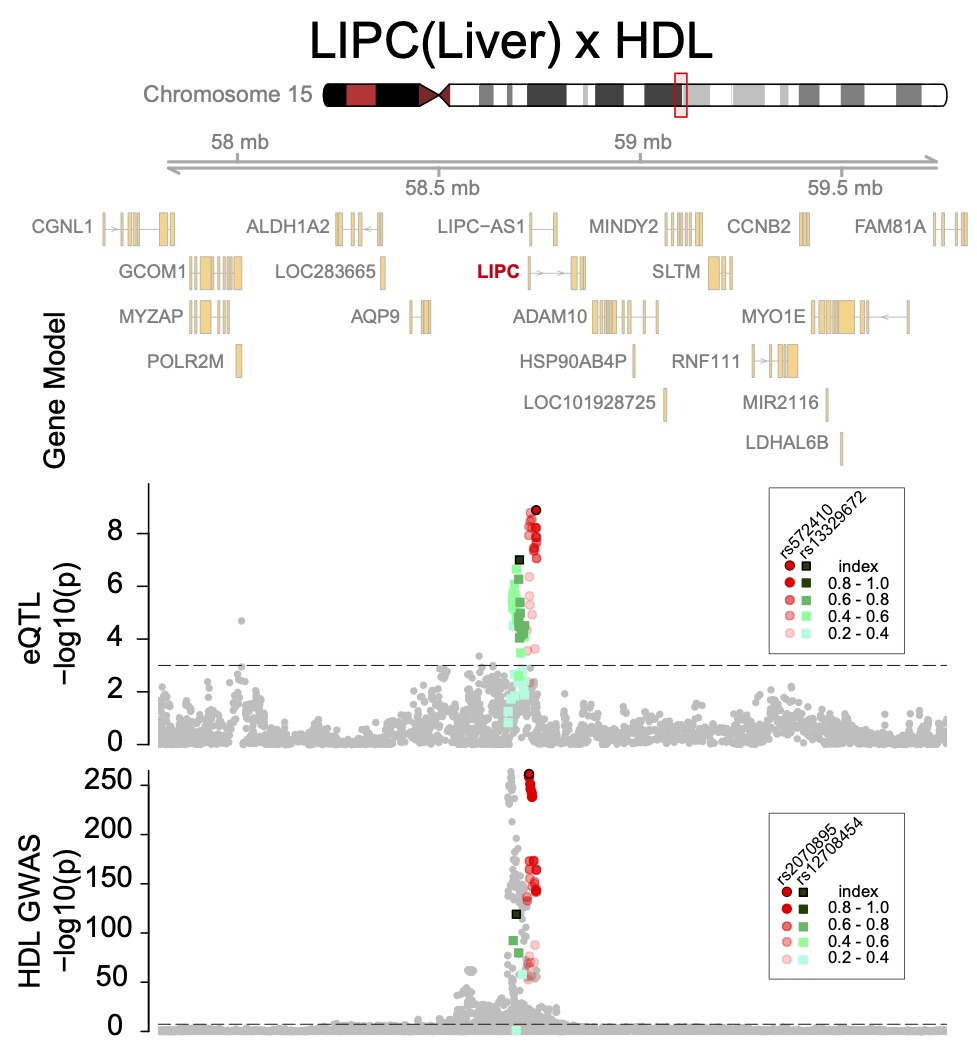
\includegraphics[width=.7\textwidth]{figs/region_lipc.jpg}
  \caption{Colocalized signals in the \emph{LIPC} region. From top
    panel to bottom, gene model (NCBI Refseq), eQTL for LIPC in liver
    (N = 588) (Strunz et al., 2018) and HDL association within UKBB (N
    = 315,133). LD was calculated to independent SNPs within 1KG EUR
    and colored accordingly. Symbols indicate independent co-localized
    ($r^2> 0.4$) eQTL-GWAS pairs. Dashed line indicates a significance
    threshold at p = 0.001 or p = 5x$10^{-8}$ for eQTL and GWAS
    respectively.} 
\end{figure}

\begin{figure}[!ht]
  \centering
  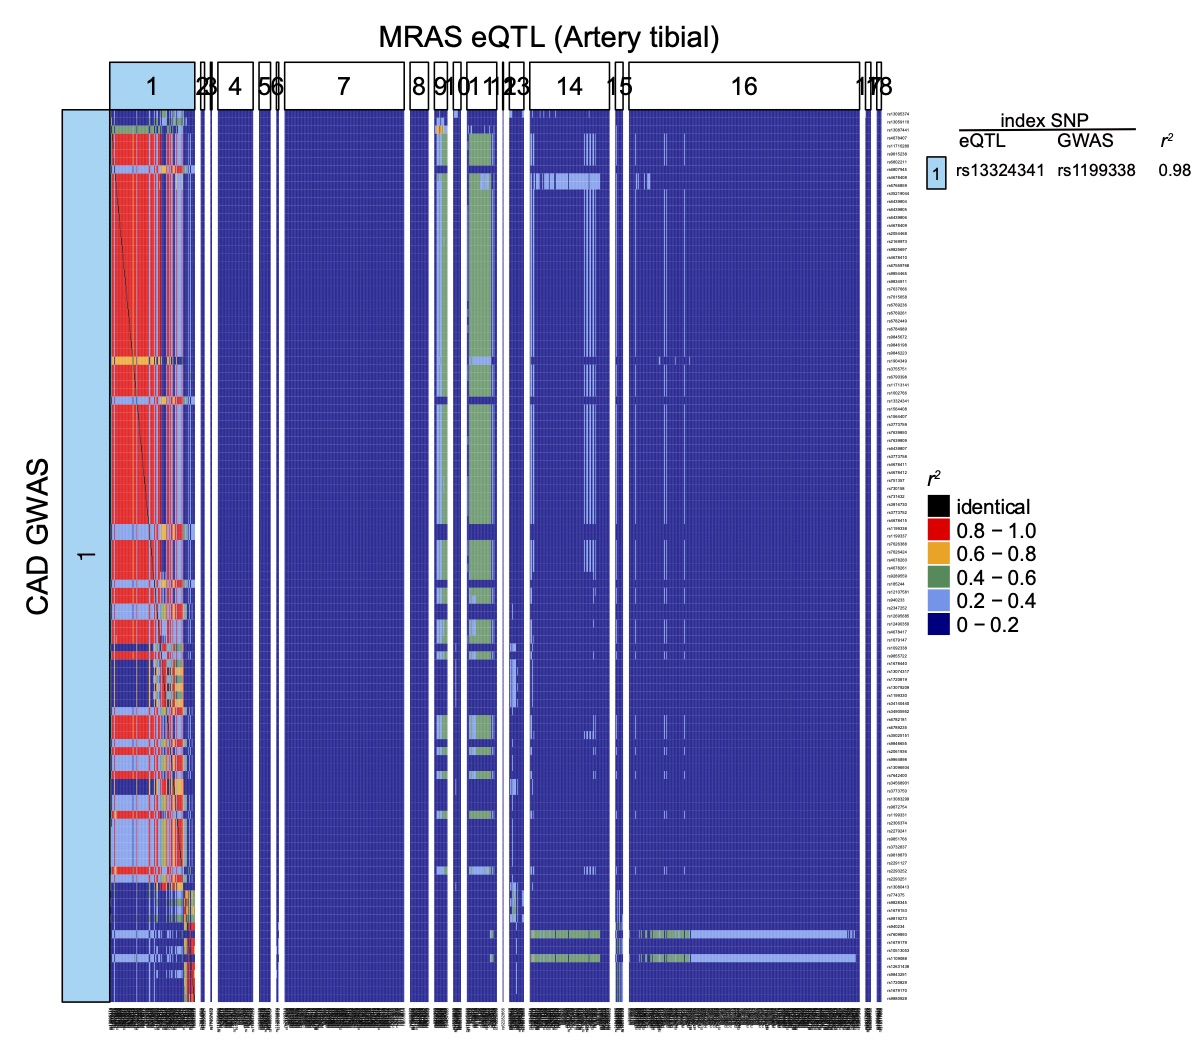
\includegraphics[width=.7\textwidth]{figs/heatmap_mras.jpg}
  \caption{LD pattern across independent clusters from \emph{MRAS}
    eQTL (Artery tibial) and CAD GWAS. LD ($r^2$) between SNPs in
    independent clumps from \emph{MRAS} in artery tibial (columns) and
    CAD GWAS SNPs (rows). Color bars at the top and left represent
    cluster (pair) ID which is sorted by base position of index eQTL
    SNPs. LD was calculated to independent SNPs within 1KG EUR and
    colored accordingly.}
  \label{fig:ld1}
\end{figure}

\begin{figure}[!ht]
  \centering
  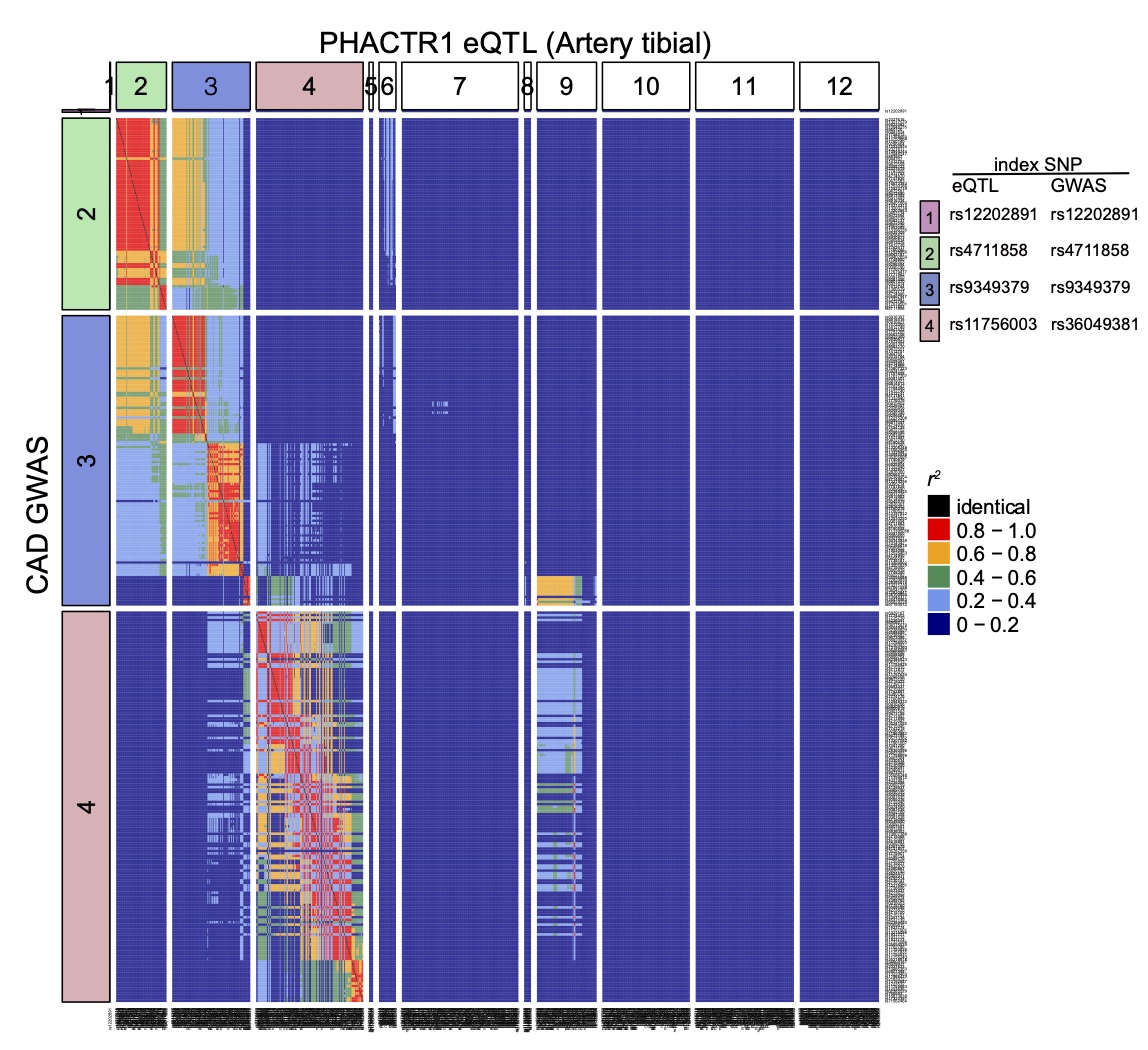
\includegraphics[width=.7\textwidth]{figs/heatmap_phactr1.jpg}
  \caption{LD pattern across independent clusters from \emph{PHACTR1}
    eQTL (Artery tibial) and CAD GWAS. LD ($r^2$) between SNPs in
    independent clumps from \emph{PHACTR1} in artery tibial (columns)
    and CAD GWAS SNPs (rows). Color bars at the top and left represent
    cluster (pair) ID which is sorted by base position of index eQTL
    SNPs. LD was calculated to independent SNPs within 1KG EUR and
    colored accordingly.} 
\end{figure}

\begin{figure}[!ht]
  \centering
  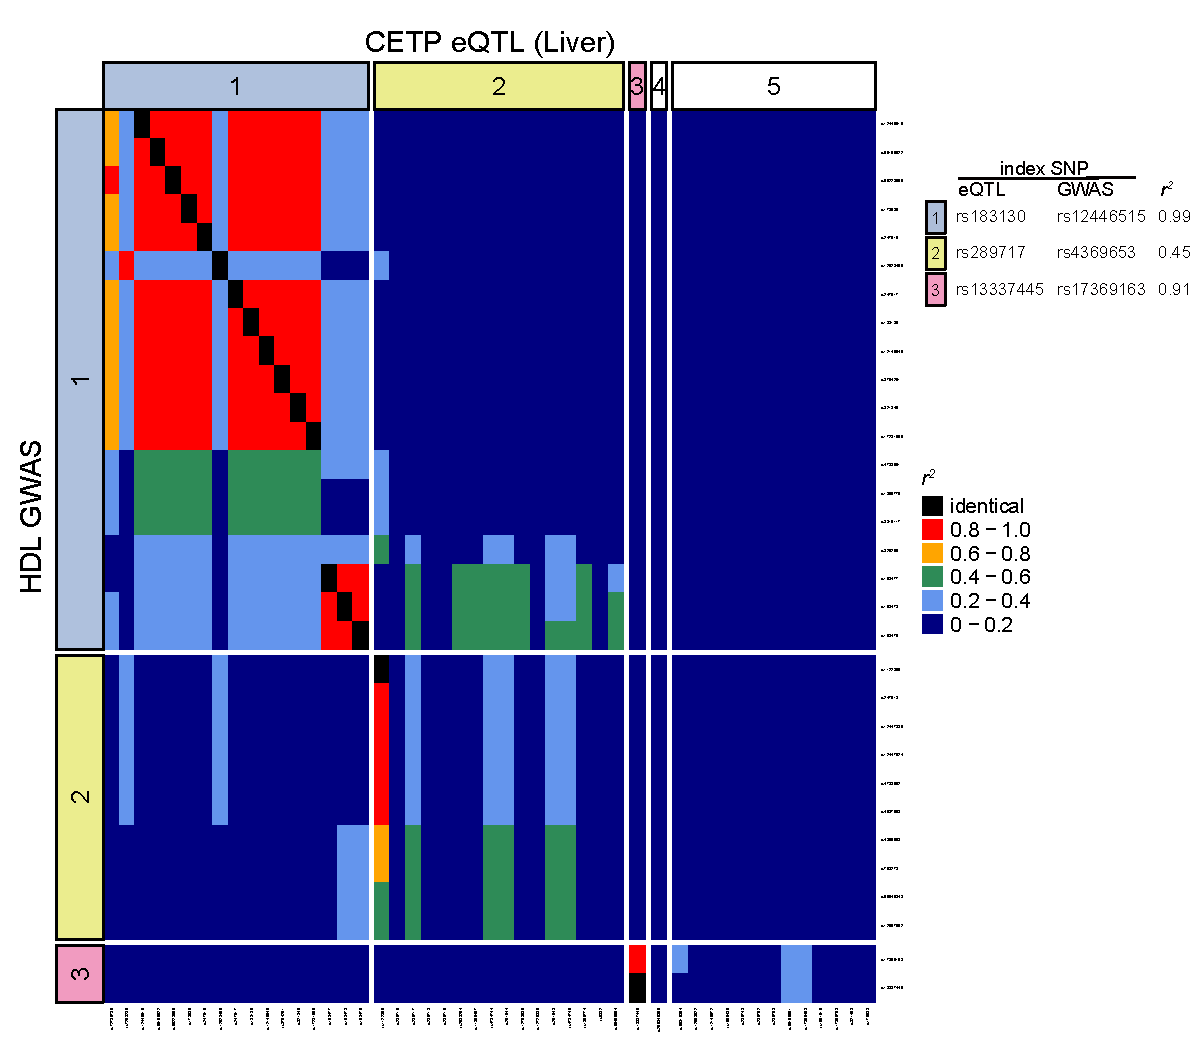
\includegraphics[width=.7\textwidth]{figs/heatmap_cetp}
  \caption{LD pattern across independent clusters from \emph{CETP}
    eQTL (liver) and HDL GWAS. LD ($r^2$) between SNPs in independent
    clumps from \emph{CETP} in liver (columns) and HDL GWAS SNPs
    (rows). Color bars at the top and left represent cluster (pair) ID
    which is sorted by base position of index eQTL SNPs. LD was
    calculated to independent SNPs within 1KG EUR and colored
    accordingly.} 
\end{figure}

\begin{figure}[!ht]
  \centering
  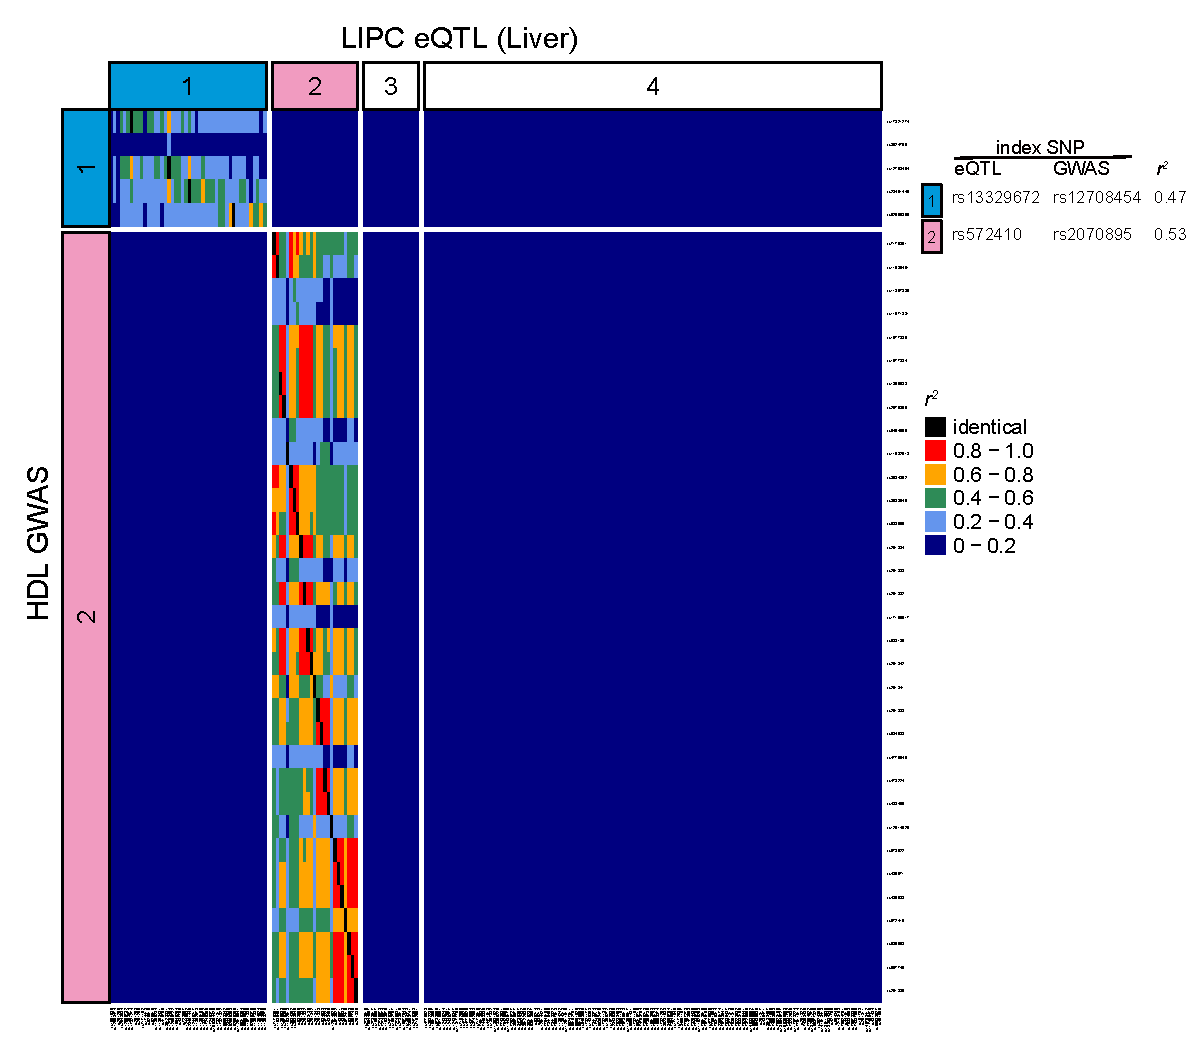
\includegraphics[width=.7\textwidth]{figs/heatmap_lipc}
  \caption{LD pattern across independent clusters from \emph{LIPC}
    eQTL (liver) and HDL GWAS. LD ($r^2$) between SNPs in independent
    clumps from \emph{LIPC} in liver (columns) and HDL GWAS SNPs
    (rows). Color bars at the top and left represent cluster (pair) ID
    which is sorted by base position of index eQTL SNPs. LD was
    calculated to independent SNPs within 1KG EUR and colored
    accordingly.} 
\end{figure}

\begin{figure}[!ht]
  \centering
  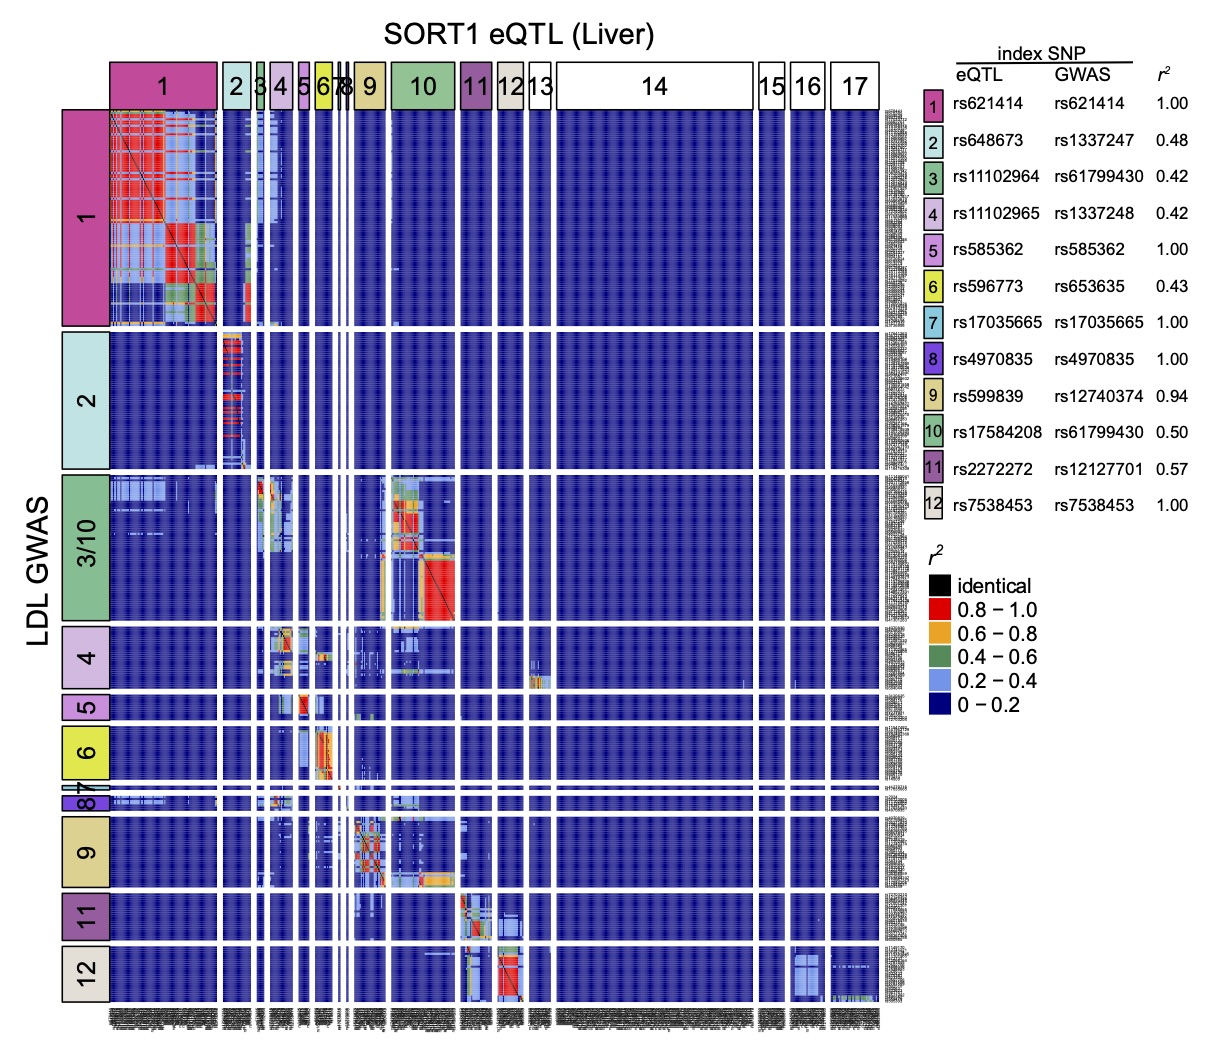
\includegraphics[width=.7\textwidth]{figs/heatmap_sort1.jpg}
  \caption{LD pattern across independent clusters from \emph{SORT1}
    eQTL (liver) and LDL GWAS. LD ($r^2$) between SNPs in independent
    clumps from \emph{SORT1} in liver (columns) and LDL GWAS SNPs
    (rows). Color bars at the top and left represent cluster (pair) ID
    which is sorted by base position of index eQTL SNPs. LD was
    calculated to independent SNPs within 1KG EUR and colored
    accordingly.}
  \label{fig:ld5}
\end{figure}

\begin{figure}[!ht]
  \centering
  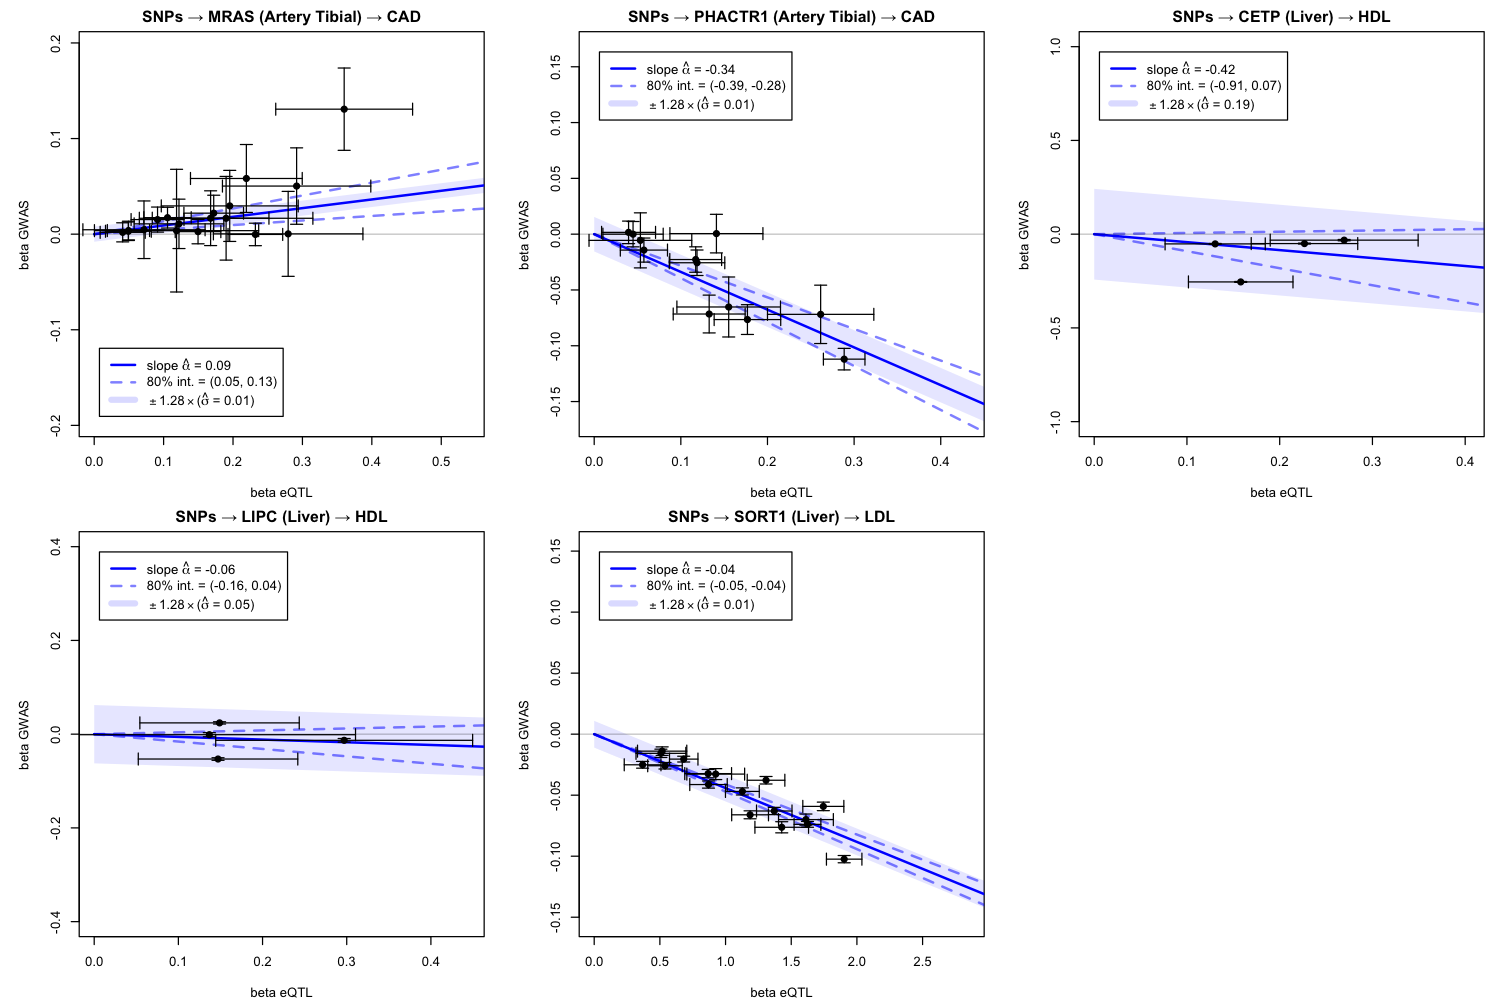
\includegraphics[width=\textwidth]{figs/realloci.png}
  \caption{MRLocus plots for the four additional gene-trait pairs, in
    addition to \emph{SORT1} in Figure 4.}
\end{figure}

\end{document}
